\documentclass[10pt,a4paper,twoside]{scrreprt}
\usepackage[english]{babel} 
\usepackage{ctex}

\pagestyle{headings}

\addtolength{\voffset}{9mm}   %>>> moves text field down
\usepackage[latin1]{inputenc}   % Encodage ISO-8859-1.
\usepackage{graphicx}
\graphicspath{{images/}} 
\newcommand{\keyevidence}[1]{\fbox{#1}}

% Smaller italic font for marginpars
\let\oldmarginpar\marginpar
\renewcommand\marginpar[1]{\-\oldmarginpar[\raggedleft\footnotesize\it #1]%
{\raggedright\footnotesize\it #1}}

\usepackage{pgf}
\usepackage[unicode,CJKbookmarks]{hyperref}

\definecolor{webgreen}{rgb}{0,.5,0}
\definecolor{webbrown}{rgb}{.6,0,0}
\definecolor{Maroon}{cmyk}{0, 0.87, 0.68, 0.32}
\definecolor{RoyalBlue}{cmyk}{1, 0.50, 0, 0}

\usepackage{listings} 
\usepackage{makeidx}
\lstdefinelanguage{FIDOCAD} 
	{morekeywords={LI,PP,PV,TY,TE,MC,EV,EP,RP,RV,BE,SA,PA,PL,FCJ,FJC,CP,CV,%
		[FIDOCAD],[FIDOLIB]}, 
	sensitive=false, 
	morecomment=[s]{[}{]}, 
	morecomment=[s][\color{blue}]{\{}{\}}, 
	morecomment=[l][\color{violet}]{*},
	moredelim=[il][\color{violet}]{�},
} 

\lstset{language=FIDOCAD,%
	basicstyle=\small\ttfamily} 

% *******************************************************
% Hyperreferences
% *******************************************************
\hypersetup{%
    colorlinks=true, linktocpage=true, pdfstartpage=3, pdfstartview=FitV,%
    breaklinks=true, pdfpagemode=UseNone, pageanchor=true, pdfpagemode=UseOutlines,%
    plainpages=false, bookmarksnumbered, bookmarksopen=true, bookmarksopenlevel=1,%
    hypertexnames=true, pdfhighlight=/O,%hyperfootnotes=true,%nesting=true,%frenchlinks,%
    urlcolor=webbrown, linkcolor=RoyalBlue, citecolor=webgreen, %pagecolor=RoyalBlue,%
    % uncomment the following line if you want to have black links (e.g., for printing)
    %urlcolor=Black, linkcolor=Black, citecolor=Black, %pagecolor=Black,%
    pdftitle={FidoCadJ -- user manual},%
    pdfauthor={Davide Bucci},%
    pdfsubject={Comment utiliser FidoCadJ},%
    pdfkeywords={FidoCAD, FidoCadJ, CAD, electronics schematics, printed circuit boards},%
    pdfcreator={pdfLaTeX},%
    pdfproducer={LaTeX with hyperref and classicthesis}%
}
\lstset{frame=single,%
	backgroundcolor=\color{lightgray},
	keywordstyle=\color{RoyalBlue},
	breaklines=true
	}

\newcommand{\micron}{\,\mu\mathrm{m}}
\newcommand{\toprule}{\hline}

\newcommand{\midrule}{\hline}

\newcommand{\bottomrule}{\hline}

\title{\Huge\color{webbrown} FidoCadJ 0.24.1 \\ 用户手册} 


\author{Davide Bucci\\[3em]
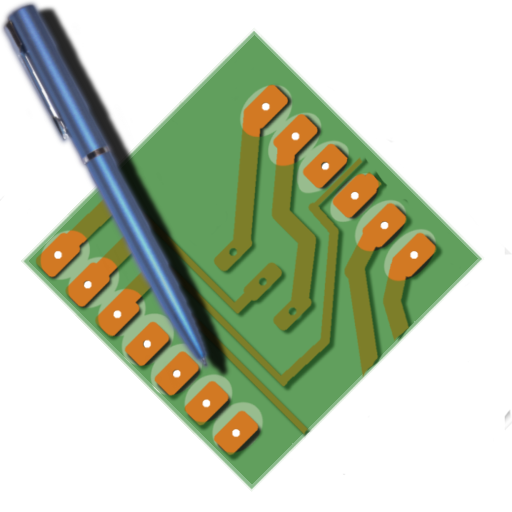
\includegraphics[width=.7\textwidth]{icona_fidocadj_a}
}

\makeindex


\begin{document}
\pagenumbering{roman}

\pdfbookmark[1]{封面}{Front}
\maketitle 

\clearpage{}
\pdfbookmark[1]{手册许可证}{Licence}

本手册的发布遵守创意公共许可证(2.5版本及以上)。以下网址可以查阅到许可证的完整内容:\\ \href{http://creativecommons.org/licenses/by-nc-nd/3.0/}{http://creativecommons.org/licenses/by-nc-nd/3.0/}

您可以自由地复制、分发、交流或展览、演示、印刷并使用本手册,但必须接受下列条件:
\begin{description}
\item [{署名}] {您必须按照作者或许可人指定的方式对手册进行署名(而不是用其它方式表明作者或许可人授权给您或授权给您使用本手册)。} 
\item [{非商业}] {您不可以把本手册用于商业。} 
\item [{禁止衍生}] {您不可以修改、转换本手册或建立基于本手册的作品。} 
\end{description}
如果您得到著作权人(Davide Bucci)的同意,可以取消上述任何限制条件。

\vfill{}
本手册中引用的所有商业名称、标志、商标都归属于注册它们的所有者。

%\begingroup 

%\let\clearpage\reax
%\let\cleardoublepage\relax
%\let\cleardoublepage\relax

%======================================= 1级标题(不加入目录)
\clearpage{}
\pdfbookmark[1]{摘要}{Abstract}
\chapter*{摘要}

本手册是FidoCadJ的官方用户手册。首先简单介绍FidoCadJ的起源和历史,接着描述它的基本使用方法。目标是让读者学会使用FidoCadJ绘制简单的电路原理图以及相应的印制电路板图。然后,详细描述FidoCadJ的格式(也可以说是FidoCad的格式)。最后,我们将给出在目前比较流行的操作系统(Linux、MacOSX和Windows)平台上下载和安装FidoCadJ的方法。

%\endgroup

%======================================= 1级标题(不加入目录)
\clearpage{}
\pdfbookmark[1]{鸣谢}{Aknowledgements}
\chapter*{鸣谢}

许多人从软件发布的第一版就开始使用了,并提出他们的意见帮助我改进此软件。在此,我要感谢it.hobby.elettronica\index{it.hobby.elettronica}新闻组\index{newsgroup}的所有参与者,是他们进行了非常富有成效的讨论。

感谢Stefano Martini耐心地在Linux系统平台上对本软件做非常仔细的测试,他是一个非常细心的alpha版本/beta版本的测试员。同时,我也要感谢Olaf Marzocchi和Emanuele Baggetta在MacOSX平台上做的测试工作。

感谢F Bertolazzi提出关于本软件使用方面的非常有用的建议,他也集成了与CadSoft Eagle\index{Eagle}兼容的库,该库用于把FidoCadJ的绘图输出给Eagle。感谢Celsius测试PCB绘图及相关元件库的功能。感谢Andrea D'Amore提出关于苹果机上FidoCadJ外观方面的建议,主要应用始于0.21.1版本。感谢Roby IZ1CYN关于库的有效论述,见本手册的~\ref{installazione_linux}~章节(关于Linux\index{Linux}系统上的安装和运行FidoCadJ的方法)。感谢Quaqua\index{Quaqua} LookAndFeel(来自Werner Randelshofer),使得苹果机用户可以享用到一个与本地系统整合地很好的FidoCadJ。同时,Werner还有一个贡献是提出许多有效的关于FidoCadJ用户界面的建议,谢谢!

本手册已经由Pasu翻译成英文,感谢他付出的工作。我也要感谢Miles(QHG007),对本手册进行仔细校对和提出一些有效的评论。

2010年4月,FidoCadJ整合进了有名的意大利网站\href{www.electroportal.it}{www.electroportal.it}。它默默地运行在服务器端,自动转换论坛用户张贴的绘图。我要表达对版主Zeno Martini、站长Nicoli Martini和该网站上其他所有用户的感激之情,是他们提出了许多实用的想法,例如FidoCadJ的批处理(这是目前跟踪到的一个很有潜力的发展方向,应该进行全面探讨)。最近,FidoReadPHP类已经完成,用于在PHP服务器上读取和解析FidoCadJ绘图。感谢Arniek和Sstrix,已经把它应用到流行的\href{www.grix.it}{www.grix.it}\index{www.grix.it}网站上,我要赞美他们!

%======================================= 1级标题(不加入目录)
\clearpage{}
\pdfbookmark[1]{FidoCadJ许可证}{License FidoCadJ}
\chapter*{FidoCadJ许可证}

版权 \copyright\ 2007-2012 Davide Bucci \href{mailto:davbucci@tiscali.it}{davbucci@tiscali.it}

本软件是自由软件:您可以在自由软件基金会公布的GUN通用公共许可证的条款下对它再发布和/或修改。

为了能够发挥软件实用价值而发布本软件,但没有任何保证,甚至没有商业或适用于特定用途的隐含保证。

您收到本软件的同时应该收到GNU公共通用许可证的一份拷贝。如果没有,请查阅:\\ \href{http://www.gnu.org/licenses/}{http://www.gnu.org/licenses/}

\clearpage{}
\pdfbookmark[1]{目录}{Table of contents}
\def\contentsname{目录}%
\tableofcontents {}

\clearpage{}
\pdfbookmark[1]{插图}{List of figures}
\def\listfigurename{插图}% 
\listoffigures

%\begingroup

%\let\clearpage\relax
%\let\cleardoublepage\relax
%\let\cleardoublepage\relax

\clearpage{}
\pdfbookmark[1]{表格}{Liste of tables}
\def\listtablename{表格}%
\listoftables

%\endgroup

%======================================= 1级标题
\chapter{介绍}

\pagenumbering{arabic}

在本章中,我们将简单介绍FidoCadJ,特别描述它的理念以及发展史。

%======================================= 2级标题
\section{FidoCadJ的理念}

FidoCad\index{FidoCad}(后面不带J)是一个矢量绘图软件,尤其适用于绘制电路原理图\index{electrical schematic}(以下简称为:原理图)和印制电路板图\index{PCB}(以下简称为:PCB图)。二十世纪九十年代后期,它在意大利Usenet社区特别流行。

FidoCad可以从Lorenzo Lutti\index{Lorenzo Lutti}的网页上自由下载(有一个Windows\index{Windows}系统上运行的意大利语版本的软件):\\ \href{http://www.enetsystems.com/~lorenzo/fidocad.asp}{http://www.enetsystems.com/\textasciitilde lorenzo/fidocad.asp}

其生成的绘图文件是一个非常紧凑的文本描述。对于在文本信息中加入绘图信息很方便,例如那些使用文本格式传输信息的Usenet群组\index{Usenet group}正需要该功能。

可惜的是,FidoCad只能运行在Windows\index{Windows}系统上。Linux系统的用户需要借助WInE\index{WInE}才能运行它。其它系统的用户,像我(我使用的是MacOSX系统)需要寻找另外的解决办法。因此,我决定对Usenet社区做一点小小的贡献,编写FidoCadJ(这里,后面加了个J)。这个软件是用纯Java\index{Java}编写的,是一个完全平台的软件。FidoCadJ可以用于显示和修改FidoCad\index{FidoCad}格式的绘图。

只要使用过FidoCad\index{FidoCad}的用户,应该很快就能够熟悉并使用FidoCadJ,因为许多命令和操作非常类似于原软件。据我了解,除了一些细节外,当前(在本手册编写时)的FidoCadJ几乎完全与原FidoCad兼容。一直以来,我都是以追求尽可能完全兼容为目标。然而,近来为了满足新用户的需求,对原格式进行了一些扩展。

FidoCadJ不同于FidoCad的其中一项特性就是它提供了导出功能。因为我是一位~\LaTeX{}~用户,我决定包含一些矢量格式的导出,其中包括Encapsulated PostScript(\textsc{EPS}\index{EPS})格式。当然,FidoCadJ可以导出非常有名的\textsc{PDF}\index{PDF}格式。另一种用于电路原理图的文件格式是CadSoft的Eagle脚本\index{CadSoft Eagle},从FidoCadJ的0.21版本开始,可以导出该格式。这样,用FidoCadJ绘制的原理图可以导出给Eagle使用。附录~\ref{specifics}~简单描述了在各个常用操作系统上安装FidoCadJ的方法。

%======================================= 2级标题
\section{FidoCadJ的历史}

我对电子电路一直都很感兴趣。当我开始关注几个电子电路方面专业的意大利Usenet新闻组\index{newsgroups}时,我注意到许多原理图是用Windows系统上的FidoCad\index{FidoCad}画的。这样就避免了使用笨拙的ASCII绘图。由于我已经多年不使用Windows了,那对我来说几乎是不可能看见它们的。我想试着做些事情来解决这个问题。\marginpar{顺便说下,我认为新做一个程序解决方案要比在原程序中增加声明不同与Windows系统的部分更好。}

开始,我学习FidoCad\index{FidoCad}的文件格式并写了一个Java\index{Java}脚本FidoReadJ\index{FidoReadJ},它能解析电路图并显示在网页中。接下来,我总是到处寻找旧帖子、网页,对其中的FidoCad文件做反向工程,做了很多。我下载过FidoCad原码,它是由Lorenzo Lutti用C++编写的,写得非常漂亮和整洁。

大约是在2007年的3月做了这些事情。几个月后,脚本就上线了,并且一部分社区人士对它进行了测试,主要集中在it.hobby.elettronica\index{it.hobby.elettronica}和it.hobby.fai-da-te\index{it.hobby.fai-da-te}网站。\footnote{FidoReadJ\index{FidoReadJ}仍然可以从这个地址获得:\\ \href{http://davbucci.chez-alice.fr/index.php?argument=elettronica/fidoreadj/fidoreadj.inc\&language=Francais}{http://davbucci.chez-alice.fr/index.php?argument=elettronica/fidoreadj/fidoreadj.inc}.}

由于我已经实现了一个FidoCad文件格式的解析器\index{interpreter},自然很有兴趣去完成一个完整的编辑器。\marginpar{其实,在1993年左右我就开始试着写一个2D矢量绘图系统。}在2008年的6、7月,分步完成了大部分的工作。FidoCadJ是一个完全重写的程序,并不是对Windows的FidoCad程序的改写或移植。

选择使用Java\index{Java}实现程序,是由于最近几年我转换使用了多种操作系统。我不再愿意花费时间和精力在不兼容的东西上了。如果只要求运行在MacOSX系统上,努力学习使用Cocoa框架,应该会获得更好的效果,但它会使FidoCadJ完全失去兼容性。我不是一个电脑迷,我愿意花时间在编程上面完全是因为我对电子电路的爱好。事实上,只要简单分析FidoCadJ源码就可以看出我不是一个纯Java\index{Java}编程和纯面向对象编程\index{Object oriented programming}的程序员。相信实现该程序会有多种更实用和更优雅的解决方案。

然而,软件并不在于选择哪种语言编写,而在于最终用户的使用体验。为此,我总是听取您的建议,以便未来更好地发展这个项目。概括来说,Java\index{Java}并不是解决各类问题的完美选择或方案。然而,我确信它的负面影响大多来自写得不好的应用程序,那些不能很好地与用户界面集成的应用程序。

由于我编程技能有限,不能做到尽善尽美,我的目标是确保FidoCadJ不会沦为一个质量差的应用程序。为此,更欢迎提出任何BUG报告和程序应用方面的建议。

2009年11月,我在SourceForge\index{SourceForge}上开了一个项目致力于FidoCadJ。那里,您可以下载到所有的可执行文件、手册和源码。您可以积极参与到FidoCadJ源码的开发工作中,这时,您需要使用Subversion(SVN)工具或SourceForge的SVN brower。项目地址:\\ \href{http://fidocadj.svn.sourceforge.net/viewvc/fidocadj/}{http://fidocadj.svn.sourceforge.net/viewvc/fidocadj/} 

如果您想来帮助我和FidoCadJ,请不要担心:您不需要是一个专业的Java程序员。您可以用一种新的语言翻译用户界面或手册、仔细检查当前手册中的矛盾和错误;您还可以从事标准库的工作\dots\ 细想一下,我给予FidoCadJ的时间中,实际只有一半是用于编程的,其余时间都用于回答用户的问题、编写和改善文档等等。在SourceForge\index{SourceForge}上,您可以加入论坛,写一个程序评论、提出改进建议或给一个BUG报告。项目首页:\\ \href{http://sourceforge.net/projects/fidocadj/}{http://sourceforge.net/projects/fidocadj/}

%======================================= 2级标题
\section{FidoCadJ的未来}

2010年4月,我偶然(几乎是个意外)登录了一个非常有名的意大利网站\href{www.electroyou.it}{www.electroyou.it}。有个用户Giancarlo Boletti,提出直接在论坛上集成一个原理图扑捉工具,类似于\LaTeX\index{LaTeX@\LaTeX}的公式。我在论坛上落了款并主动提出愿意进行合作。这样,由于他的发言引出了FidoCadJ。经过几天与站长(他是一个很不错的站长)的交流,系统准备就绪了:在有代码形式绘图的帖子中,使用一对标签实现简单地复制和粘贴功能。论坛软件调用服务器上的FidoCadJ获得代码的绘图。然后把这个绘图显示在论坛的帖子中,并且仍然可以取得绘图的代码。这样,如果他只是浏览而不是修改的话,不需要安装任何插件,并且他还可以通过很少的鼠标点击动作取得绘图代码。

Figure~\ref{fig_discussione_electroyou}~显示了\href{www.electroyou.it}{www.electroyou.it}上我的帖子的一部分。这个系统是如此强大和灵活,以至于用户对它表现出的热情令我感到了前所未有的惊讶!\footnote{如果您能阅读意大利文,这里有一篇我写的文章:\\ \href{http://www.electroyou.it/darwinne/wiki/fidocadj}{http://www.electroyou.it/darwinne/wiki/fidocadj}	 }
 	 
\begin{figure}
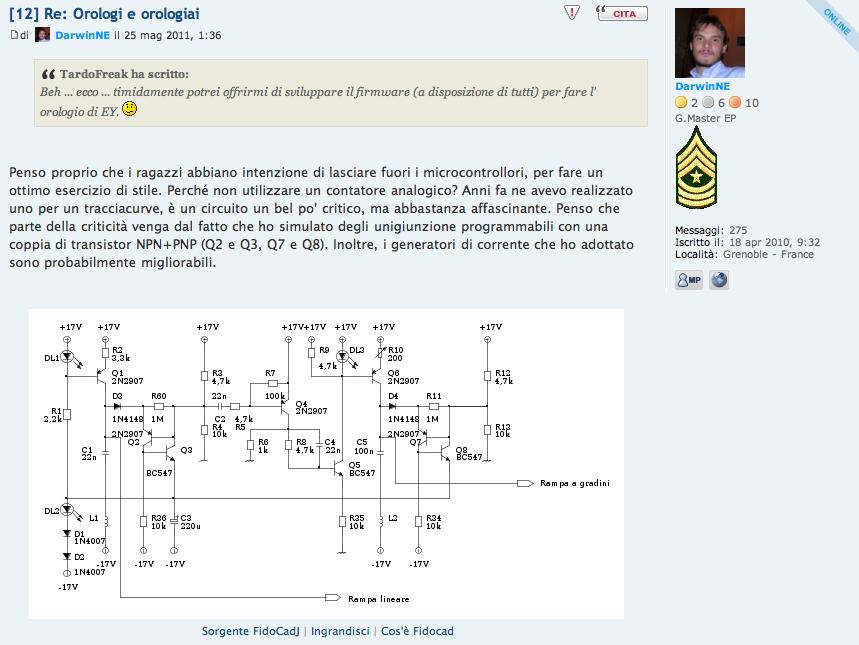
\includegraphics[width=\textwidth]{discussione_electroyou.png}
\caption{\href{www.electroyou.it}{www.electroyou.it}\index{www.electroyou.it}上我的帖子的一部分。您只需要用鼠标点击一个图标就可以缩放查看原理图。点击另一个图标就可以立即得到绘图代码,并可以把代码复制/粘贴到FidoCadJ中进行修改。}
\label{fig_discussione_electroyou}
\end{figure}

FidoCadJ在\href{www.electroyou.it}{www.electroyou.it}\index{www.electroyou.it}上取得了成功,激发了其它平台上实现类似系统的一些需求,特别是\href{www.grix.it}{www.grix.it}\index{www.grix.it},另一个众所周知的意大利电子专业网站。该网站的服务器无法运行Java程序,于是就有了FidoReadPHP类。它可以运行在PHP服务器上,取得FidoCadJ绘图代码的图形。FidoReadPHP项目是开放源码的,可以从SourceForge上获得:\\ \href{https://sourceforge.net/projects/fidoreadphp/}{https://sourceforge.net/projects/fidoreadphp/}

尽管PHP的图形能力与Java相比是相当有限的,但从获得的图形效果来看还是可以的,类似于从\href{www.electroyou.it}{www.electroyou.it}上获得的图形\footnote{再次,如果您能阅读意大利文,这里有篇文章:\\ \href{http://www.grix.it/viewer.php?page=9335}{http://www.grix.it/viewer.php?page=9335}}。Figure~\ref{fig_fidocadj_grix3}显示了一个FidoReadPHP绘制的图形。

\begin{figure}
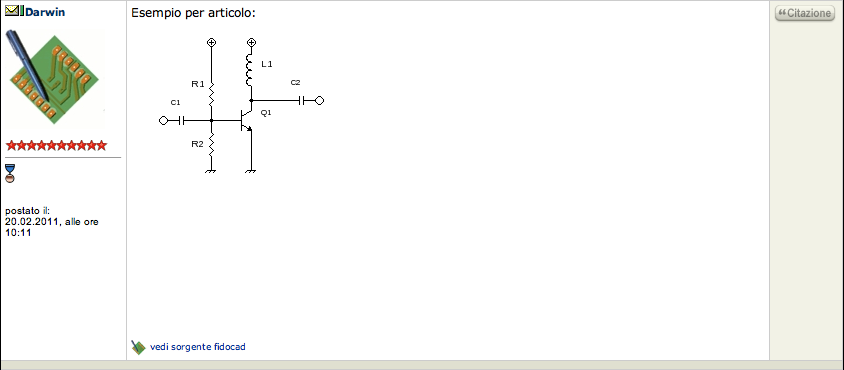
\includegraphics[width=\textwidth]{fidocadj_grix3.png}
\caption{\href{www.grix.it}{www.grix.it}\index{www.grix.it}论坛上整合了FidoCadJ绘图帖子的示例,您只需要一次鼠标点击就可以取得绘图代码。}
\label{fig_fidocadj_grix3}
\end{figure}

我认为FidoCadJ的未来,不是变得更加复杂,发展成一个完整的电子CAD。发展与讨论组和论坛的整合可能更加理想,经验表明了这种可能性,而且已经激起了用户的热情。

%======================================= 1级标题
\chapter{FidoCadJ绘图}

对那些原来用过矢量绘图\index{vectorial drawing}软件的用户来说,FidoCadJ应该是凭经验就能使用的软件。图~\ref{fig_fidocadj}~显示了本软件在MacOSX\index{MacOSX}系统上运行的一个截屏\marginpar{专业的苹果用户会注意到窗口的布局很合理!}。在其它系统上运行的外观(例如,图~\ref{fig_metal}~显示了在Sun/Oracle\index{Sun/Oracle}系统上运行的外观,设置为Metal\index{Metal} LookAndFeel)可能会有些细微的差别,但操作理念是一致的。我们将会发现该绘图软件的特点是利用基本图形元件(以下简称为:基元件)\index{primitive}组合成一张绘图。

\begin{figure}
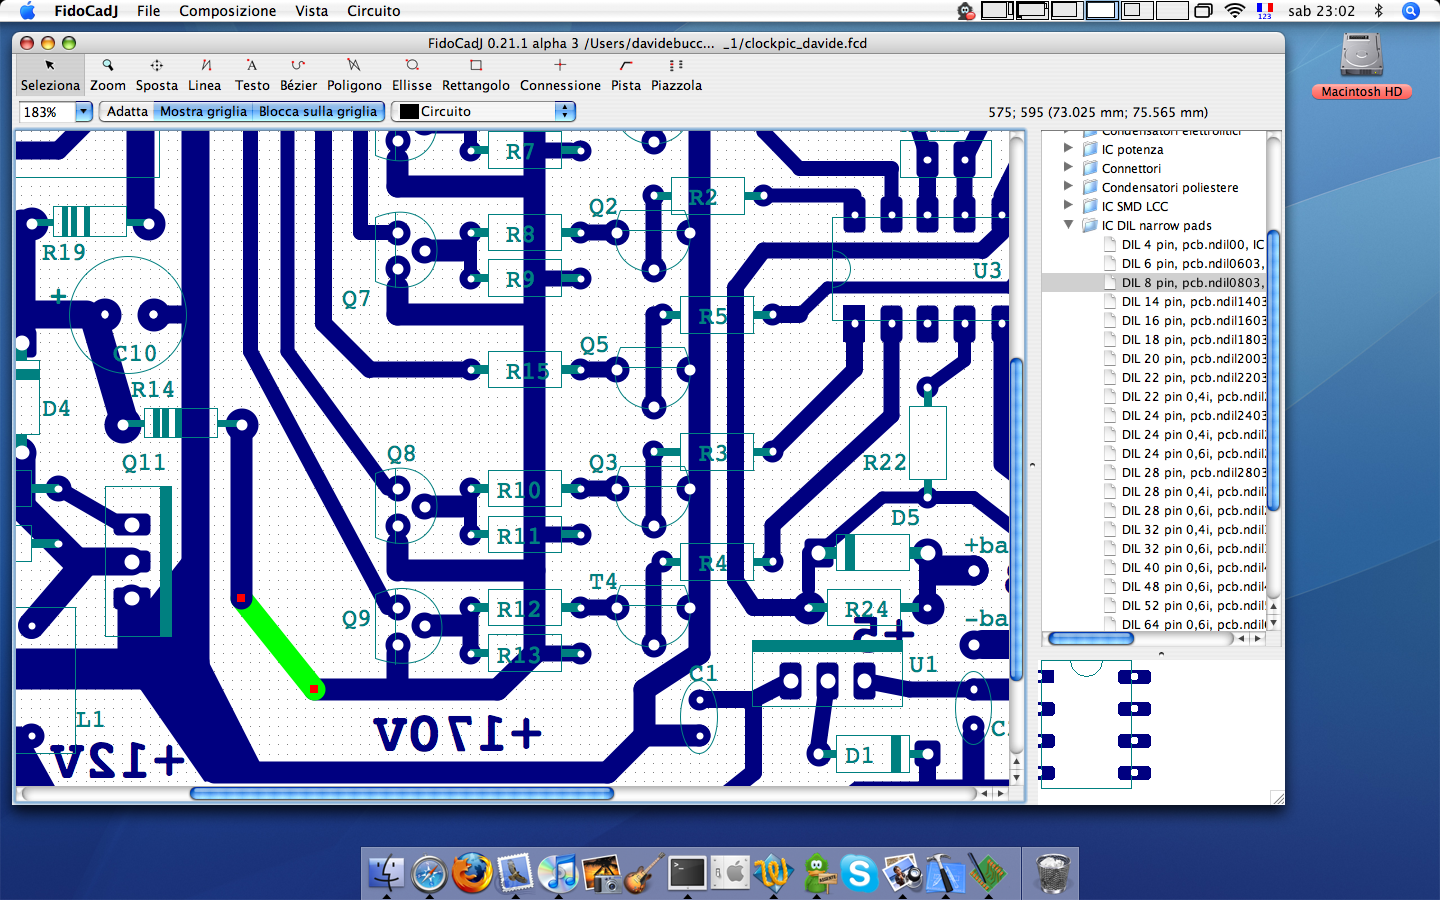
\includegraphics[width=1\textwidth]{fidocadj_macosx.png} 
\caption{运行在MacOSX Tiger\index{MacOSX}系统上的FidoCadJ的典型界面。附录~\ref{specifics}介绍苹果机\index{Macintosh}操作系统的特性。}
\label{fig_fidocadj} 
\end{figure}

\begin{figure}
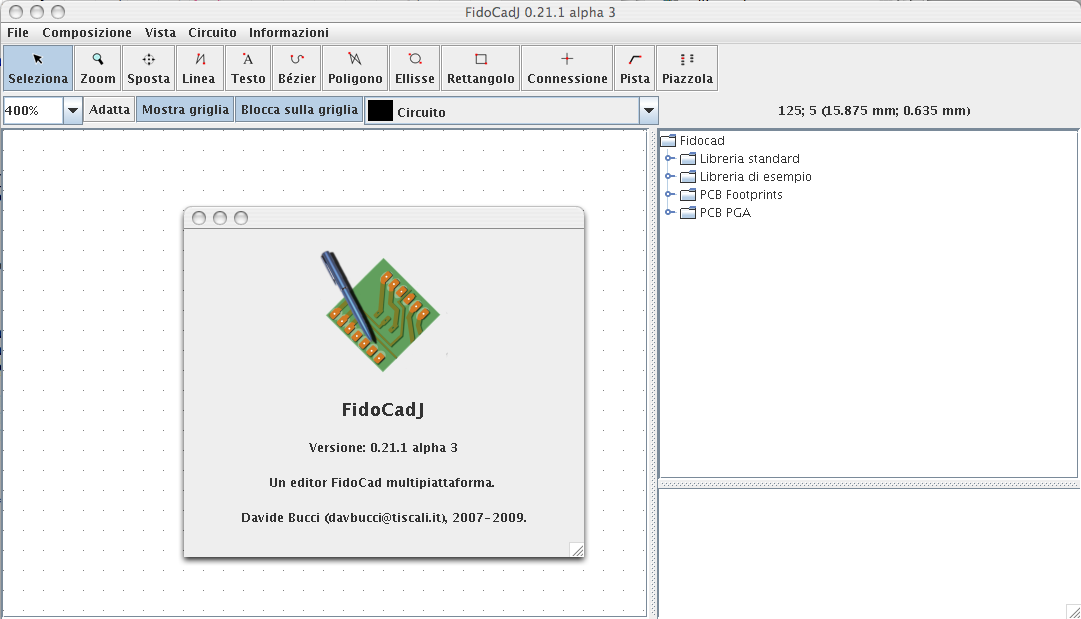
\includegraphics[width=1\textwidth]{fidocadj_metal.png} 
\caption{FidoCadJ的Metal\index{Metal} LookAndFeel}
\label{fig_metal} 
\end{figure}

%======================================= 2级标题
\section{绘图工具}

我们可以在工具栏\index{toolbar}(位于窗口顶部)上找到常用的工具,用来创建和编辑绘图。表~\ref{tab_comandi}~简要汇总了这些工具的功能、命令和关联动作。你会发现,一旦按下一个工具栏按钮,它会保持在按下状态,直到按下另一个工具栏按钮\marginpar{设计这种操作方式的灵感来自于七十年代非常流行的老式真空管收音机的开关方式。}。我们可以从工具栏上选择需要使用的基元件\index{primitive}\footnote{更多关于绘图元件的介绍请见~\ref{sec_primitive}~章节。}。靠工具栏的右边,有个下拉菜单显示了当前的工作层(见~\ref{sec_layer}~章节,有更多的说明)。

工具栏\index{command bar}可以部分定制。特别是,我们可以定制按钮的外观(显示图标或显示图标和文本;显示图标也有两种方式可供选择)。我们可以通过菜单{}“文件/选项”来改变这些设置\footnote{MacOSX系统例外,在FidoCadJ菜单的{}”Preferences”里改变设置。}。任何设置的改变都要重新启应用程序后才会生效,以后我们可能经常要改变一些设置,会证实这一点。图~\ref{fig_fidocadj}~和图~\ref{fig_metal}~显示的工具栏(位于窗口标题栏的下方)是设置成文本和小图标的显示方式。工具栏的第二排靠左边,我们可以看到缩放比例设置和按钮{}“适合窗口”、{}“显示网格”和{}“对齐到网格”。第一个“适合窗口”按钮,可以自动调节到最合适的比例,以在窗口中最大化显示整张绘图。第二个”显示网格”按钮,可以切换网格可见或不可见。第三个“对齐到网格”按钮,可以设置在绘制元件时是否对齐到附近的网格。如果需要把元件对整齐,您可以按住~\keyevidence{Alt}~键的同时使用方向键来移动选中的元件。

\begin{table}
\centering
\begin{tabular}{clp{0.5\textwidth}}
\toprule 
快捷键 & 命令  & 使用方法\tabularnewline
\midrule
\keyevidence{A} 或 \keyevidence{空格} & \raisebox{-.2em}{
\includegraphics[width=1em]{icons/arrow}}\textsc{选择}\index{selection}  & 选择一个或多个元件。按住~\keyevidence{Control~}键(MacOSX系统中是~\keyevidence{Command}~键)进行多选,或从多选中去掉一个。也可以框选多个元件。按~\keyevidence{R}~键旋转选择的元件;按~\keyevidence{S}~键翻转选择的元件。双击一个元件可以修改它的属性。\tabularnewline
 & \raisebox{-.2em}{
\includegraphics[width=1em,]{icons/magnifier}}\textsc{缩放}\index{zoom}  & 左键点击放大;右键点击缩小。\tabularnewline
 & \raisebox{-.2em}{
\includegraphics[width=1em,]{icons/move}}\textsc{浏览}\index{move}  & 在图纸上左键点击并移动鼠标可以移动绘图。\tabularnewline
\keyevidence{L}  & \raisebox{-.2em}{
\includegraphics[width=1em,]{icons/line}}\textsc{直线}\index{line}  & 画一条或多条连续直线。双击或按~\keyevidence{Esc}~键完成绘制。\tabularnewline %\footnote{In FidoCadJ versions prior to 0.20.5, a right click would switch to the ``Select'' mode}
\keyevidence{T}  & \raisebox{-.2em}{
\includegraphics[width=1em,]{icons/text}}\textsc{文本}\index{text}  & 放置一个文本。\tabularnewline
\keyevidence{B}  & \raisebox{-.2em}{
\includegraphics[width=1em,]{icons/bezier}}\textsc{贝塞尔曲线}\index{B�zier}  & 画一条贝塞尔曲线。\tabularnewline
\keyevidence{P}  & \raisebox{-.2em}{
\includegraphics[width=1em,]{icons/polygon}}\textsc{多边形}\index{polyline}  & 画一个多边形(填充或不填充)。双击或按~\keyevidence{Esc}~键完成绘制。\tabularnewline
\keyevidence{K} & \raisebox{-.2em}{
\includegraphics[width=1em]{icons/complexcurve}}\textsc{曲线}\index{curve} & 画一条开放或闭合的自然三次样条曲线。双击或按~\keyevidence{Esc}~键完成绘制。\tabularnewline
\keyevidence{E}  & \raisebox{-.2em}{
\includegraphics[width=1em,]{icons/ellipse}}\textsc{椭圆}\index{ellipse}  & 画一个椭圆(填充或不填充)(按住~\keyevidence{Control}~键:画圆形)。\tabularnewline
\keyevidence{G}  & \raisebox{-.2em}{
\includegraphics[width=1em,]{icons/rectangle}}\textsc{矩形}\index{rectangle}  & 画一个矩形(填充或不填充)。\tabularnewline
\keyevidence{C}  & \raisebox{-.2em}{
\includegraphics[width=1em,]{icons/connection}}\textsc{连接点}\index{junction}  & 画一个电气连接点。\tabularnewline
\keyevidence{I}  & \raisebox{-.2em}{
\includegraphics[width=1em,]{icons/pcbline}}\textsc{PCB导线}\index{PCB track}  & 画一条PCB导线。通过菜单{}“文件/选项”打开的对话框可以修改默认宽度。\tabularnewline
\keyevidence{Z}  & \raisebox{-.2em}{
\includegraphics[width=1em,]{icons/pcbpad}}\textsc{PCB焊盘}\index{PCB pad@\textsc{PCB }pad}  &  画一个PCB焊盘。通过菜单{}”文件/选项”打开的对话框可以修改默认尺寸。\tabularnewline
\bottomrule
\end{tabular}
\caption{FidoCadJ绘图命令汇总表。最左边的“快捷键”栏给出快速选择该命令的按键。在元件放置模式时,右键点击任何已绘制的元件可以打开相应的属性窗口。}
\label{tab_comandi} 
\end{table}

窗口右边有一个树形列表,列出应用程序加载的元件库(库中的元件称为:宏图形元件\index{macro},以下简称:为宏元件)。要在绘图中加入一个的宏元件,我们只需要从列表中选择它,然后在绘图中左键点击即可。FidoCadJ\index{FidoCad}默认加载库中包含绘制原理图\index{electrical schematic}所需使用的所有标准符号和绘制PCB图所需使用的大多数封装\index{PCB!footprint}。

从版本0.22开始,您可以在FidoCadJ载入的元件库中进行快速搜索\index{Quick research}。您只需要在搜索框中键入一些字符,就会在树形列表的已加载库中进行匹配(见图~\ref{fig_ricerca}~),此时可以使用向上和向下按键在匹配项间移动。

\begin{figure}
\centering
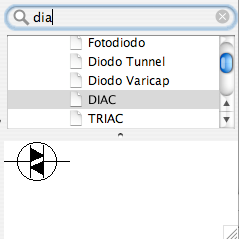
\includegraphics[width=.4\textwidth]{ricerca}
\caption{在加载库中快速查找。}
\label{fig_ricerca}
\end{figure}
\begin{figure}
\centering 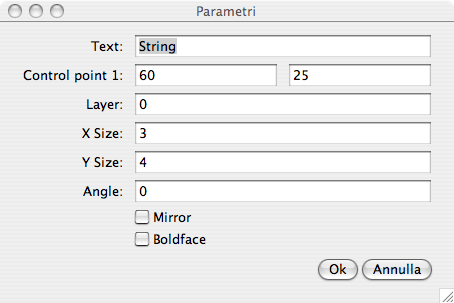
\includegraphics[width=0.7\textwidth,]{param_testo} 
\caption{FidoCadJ绘图的文本元件参数设置对话框。}
\label{fig_param_testo} 
\end{figure}

图~\ref{fig_param_testo}~显示了一个在选择模式\index{selection}时双击已绘制元件得到的参数设置对话框(这里是文本元件的参数设置对话框)。任何一个已绘制元件都可以通过这样的对话框修改所有属性(如坐标、旋转、\dots)。由于各种元件的设置参数不同,随着选择的元件不同,参数设置对话框显示的内容也是不同的。

%======================================= 2级标题
\section{一张简单的原理图}

我们将展示如何绘制一张图~\ref{fig_schema}~所示的简单的原理图,作为使用该应用程序的一个例子。

\begin{figure}
\centering %\includegraphics[width=.5\textwidth]{schema}
\begin{pgfpicture}{0cm}{0cm}{125pt}{111pt}
% Created by FidoCadJ ver. 0.21, export filter by Davide Bucci
\pgfsetxvec{\pgfpoint{1pt}{0pt}}
\pgfsetyvec{\pgfpoint{0pt}{1pt}}
\pgfsetlinewidth{0.33pt}
\pgfsetroundjoin 
\pgftranslateto{\pgfxy(0,111)}
\begin{pgfmagnify}{1}{-1}
% Layer color definitions
\definecolor{layer0}{rgb}{0.0,0.0,0.0}
\definecolor{layer1}{rgb}{0.0,0.0,0.5}
\definecolor{layer2}{rgb}{1.0,0.0,0.0}
\definecolor{layer3}{rgb}{0.0,0.5,0.5}
\definecolor{layer4}{rgb}{1.0,0.78,0.0}
\definecolor{layer5}{rgb}{1.0,0.78,0.0}
\definecolor{layer6}{rgb}{1.0,0.78,0.0}
\definecolor{layer7}{rgb}{1.0,0.78,0.0}
\definecolor{layer8}{rgb}{1.0,0.78,0.0}
\definecolor{layer9}{rgb}{1.0,0.78,0.0}
\definecolor{layer10}{rgb}{1.0,0.78,0.0}
\definecolor{layer11}{rgb}{1.0,0.78,0.0}
\definecolor{layer12}{rgb}{1.0,0.78,0.0}
\definecolor{layer13}{rgb}{1.0,0.78,0.0}
\definecolor{layer14}{rgb}{1.0,0.78,0.0}
\definecolor{layer15}{rgb}{1.0,0.78,0.0}
% End of color definitions
\color{layer0}
\pgfline{\pgfxy(100,67)}{\pgfxy(105,70)}
\pgfline{\pgfxy(90,65)}{\pgfxy(100,65)}
\pgfline{\pgfxy(100,60)}{\pgfxy(100,70)}
\pgfline{\pgfxy(105,60)}{\pgfxy(105,55)}
\pgfline{\pgfxy(100,63)}{\pgfxy(105,60)}
\pgfline{\pgfxy(105,70)}{\pgfxy(105,75)}
\pgfmoveto{\pgfxy(103,70)}
\pgflineto{\pgfxy(104,68)}
\pgflineto{\pgfxy(105,70)}
\pgfclosepath 
\pgffill 
\begin{pgfmagnify}{1}{-1}
\pgfputat{\pgfxy(110,-55)}{\pgfbox[left,top]{\footnotesize{Q1B}}}
\end{pgfmagnify}
\begin{pgfmagnify}{1}{-1}
\pgfputat{\pgfxy(110,-65)}{\pgfbox[left,top]{\footnotesize{LM394}}}
\end{pgfmagnify}
\pgfline{\pgfxy(40,67)}{\pgfxy(35,70)}
\pgfline{\pgfxy(50,65)}{\pgfxy(40,65)}
\pgfline{\pgfxy(40,60)}{\pgfxy(40,70)}
\pgfline{\pgfxy(35,60)}{\pgfxy(35,55)}
\pgfline{\pgfxy(40,63)}{\pgfxy(35,60)}
\pgfline{\pgfxy(35,70)}{\pgfxy(35,75)}
\pgfmoveto{\pgfxy(37,70)}
\pgflineto{\pgfxy(36,68)}
\pgflineto{\pgfxy(35,70)}
\pgfclosepath 
\pgffill 
\begin{pgfmagnify}{1}{-1}
\pgfputat{\pgfxy(10,-55)}{\pgfbox[left,top]{\footnotesize{Q1A}}}
\end{pgfmagnify}
\begin{pgfmagnify}{1}{-1}
\pgfputat{\pgfxy(0,-65)}{\pgfbox[left,top]{\footnotesize{LM394}}}
\end{pgfmagnify}
\pgfline{\pgfxy(50,65)}{\pgfxy(90,65)}
\pgfline{\pgfxy(35,75)}{\pgfxy(35,95)}
\pgfline{\pgfxy(105,75)}{\pgfxy(105,95)}
\pgfline{\pgfxy(35,40)}{\pgfxy(35,55)}
\pgfline{\pgfxy(35,30)}{\pgfxy(35,32)}
\pgfmoveto{\pgfxy(36,32)}
\pgflineto{\pgfxy(34,32)}
\pgflineto{\pgfxy(34,38)}
\pgflineto{\pgfxy(36,38)}
\pgfclosepath 
\pgfqstroke 
\pgfline{\pgfxy(35,38)}{\pgfxy(35,40)}
\begin{pgfmagnify}{1}{-1}
\pgfputat{\pgfxy(45,-40)}{\pgfbox[left,top]{}}
\end{pgfmagnify}
\begin{pgfmagnify}{1}{-1}
\pgfputat{\pgfxy(45,-35)}{\pgfbox[left,top]{}}
\end{pgfmagnify}
\pgfline{\pgfxy(35,15)}{\pgfxy(35,30)}
\pgfline{\pgfxy(25,15)}{\pgfxy(35,15)}
\pgfline{\pgfxy(25,15)}{\pgfxy(23,15)}
\pgfellipse[stroke]{\pgfxy(21.0,15.0)}{\pgfxy(2.0,0)}{\pgfxy(0,2.0)}
\pgfline{\pgfxy(22,15)}{\pgfxy(20,15)}
\pgfline{\pgfxy(21,16)}{\pgfxy(21,14)}
\begin{pgfmagnify}{1}{-1}
\pgfputat{\pgfxy(35,-25)}{\pgfbox[left,top]{}}
\end{pgfmagnify}
\begin{pgfmagnify}{1}{-1}
\pgfputat{\pgfxy(35,-20)}{\pgfbox[left,top]{}}
\end{pgfmagnify}
\pgfline{\pgfxy(35,50)}{\pgfxy(55,50)}
\pgfline{\pgfxy(55,50)}{\pgfxy(55,65)}
\pgfcircle[fill]{\pgfxy(55,65)}{1pt}\pgfcircle[fill]{\pgfxy(35,50)}{1pt}\pgfline{\pgfxy(105,45)}{\pgfxy(105,55)}
\pgfline{\pgfxy(105,35)}{\pgfxy(105,40)}
\pgfline{\pgfxy(105,25)}{\pgfxy(105,30)}
\pgfline{\pgfxy(35,95)}{\pgfxy(35,100)}
\pgfline{\pgfxy(32,100)}{\pgfxy(38,100)}
\pgfline{\pgfxy(33,101)}{\pgfxy(37,101)}
\pgfline{\pgfxy(34,102)}{\pgfxy(36,102)}
\begin{pgfmagnify}{1}{-1}
\pgfputat{\pgfxy(45,-105)}{\pgfbox[left,top]{}}
\end{pgfmagnify}
\begin{pgfmagnify}{1}{-1}
\pgfputat{\pgfxy(45,-100)}{\pgfbox[left,top]{}}
\end{pgfmagnify}
\pgfline{\pgfxy(105,95)}{\pgfxy(105,100)}
\pgfline{\pgfxy(102,100)}{\pgfxy(108,100)}
\pgfline{\pgfxy(103,101)}{\pgfxy(107,101)}
\pgfline{\pgfxy(104,102)}{\pgfxy(106,102)}
\begin{pgfmagnify}{1}{-1}
\pgfputat{\pgfxy(115,-105)}{\pgfbox[left,top]{}}
\end{pgfmagnify}
\begin{pgfmagnify}{1}{-1}
\pgfputat{\pgfxy(115,-100)}{\pgfbox[left,top]{}}
\end{pgfmagnify}
\begin{pgfmagnify}{1}{-1}
\pgfputat{\pgfxy(40,-30)}{\pgfbox[left,top]{\footnotesize{10 k}}}
\end{pgfmagnify}
\begin{pgfmagnify}{1}{-1}
\pgfputat{\pgfxy(110,-45)}{\pgfbox[left,top]{\footnotesize{I}}}
\end{pgfmagnify}
\pgfmoveto{\pgfxy(105,55)}
\pgflineto{\pgfxy(104,53)}
\pgflineto{\pgfxy(106,53)}
\pgfclosepath 
\pgffill 
\pgfline{\pgfxy(105,55)}{\pgfxy(105,50)}
\begin{pgfmagnify}{1}{-1}
\pgfputat{\pgfxy(115,-60)}{\pgfbox[left,top]{}}
\end{pgfmagnify}
\begin{pgfmagnify}{1}{-1}
\pgfputat{\pgfxy(115,-55)}{\pgfbox[left,top]{}}
\end{pgfmagnify}
\end{pgfmagnify}
\end{pgfpicture} 
\caption{参考原理图:NPN三极管的一个电路镜像。}
\label{fig_schema} 
\end{figure}

FidoCadJ运行起来后,我们可以通过菜单“文件/新建”来创建一个新的绘图。

围绕要建立的原理图,首先,我们要在绘图区域放置2个晶体管\index{transistor}。此时,我们需要标准库\index{standard library}中的宏元件(标准库是默认加载的,位于窗口的右侧)。所需宏元件的名称为{}“NPN transistor”,它在{}“Standard library”的{}“Diodes and transistors”类型中。通过左键点击宏元\index{macro}件的名称选择它,然后在绘图区域中的任何想要放置的位置处再次左键点击就可以绘制它(选择绘制位置时,FidoCadJ会显示一个宏元件的预览)。到此,我们的绘图应该类似于图~\ref{fig_fidocadj_fase1}~所示的样子。

\begin{figure}
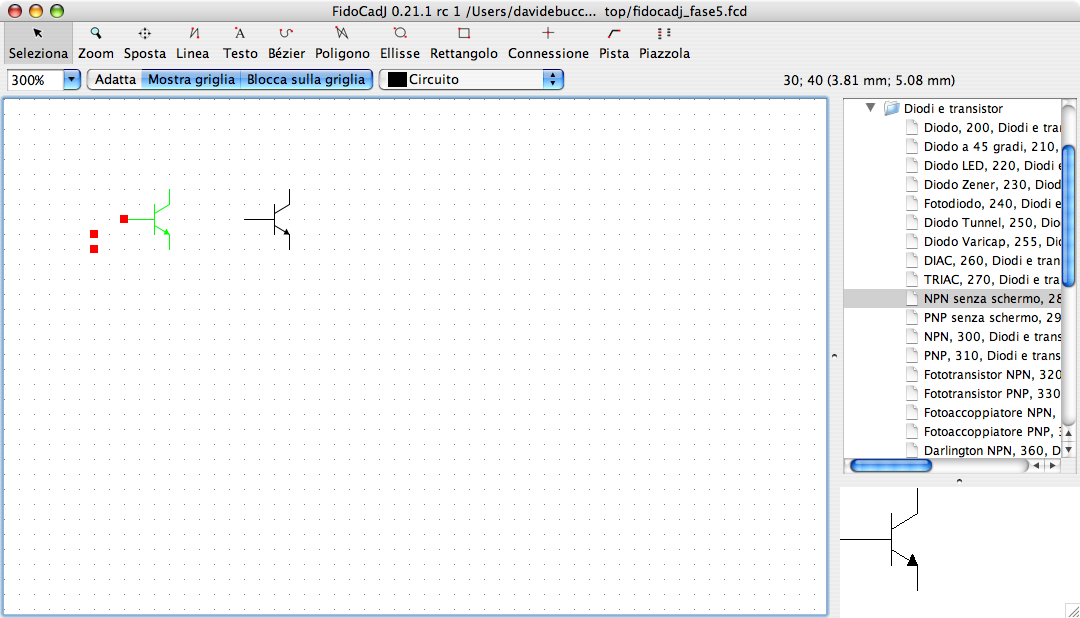
\includegraphics[width=1\textwidth,]{fidocadj_fase1} 
\caption{首先,我们画一对三极管。}
\label{fig_fidocadj_fase1} 
\end{figure}

我们注意到左边的双极型晶体管的方向不对。为了解决这个问题,左键点击工具栏上的{}”选择”工具并点击选择那个晶体管(选中后,晶体管会呈现绿色高亮显示状态,并带有3个红色小正方形控制点\index{control point}),然后按~\keyevidence{S}~键把它翻转。你也可以在选择了宏元件并在绘图中绘制前按~\keyevidence{S}~键。到此,我们的绘图应该类似于图~\ref{fig_fidocadj_fase2}~所示的样子。

\begin{figure}
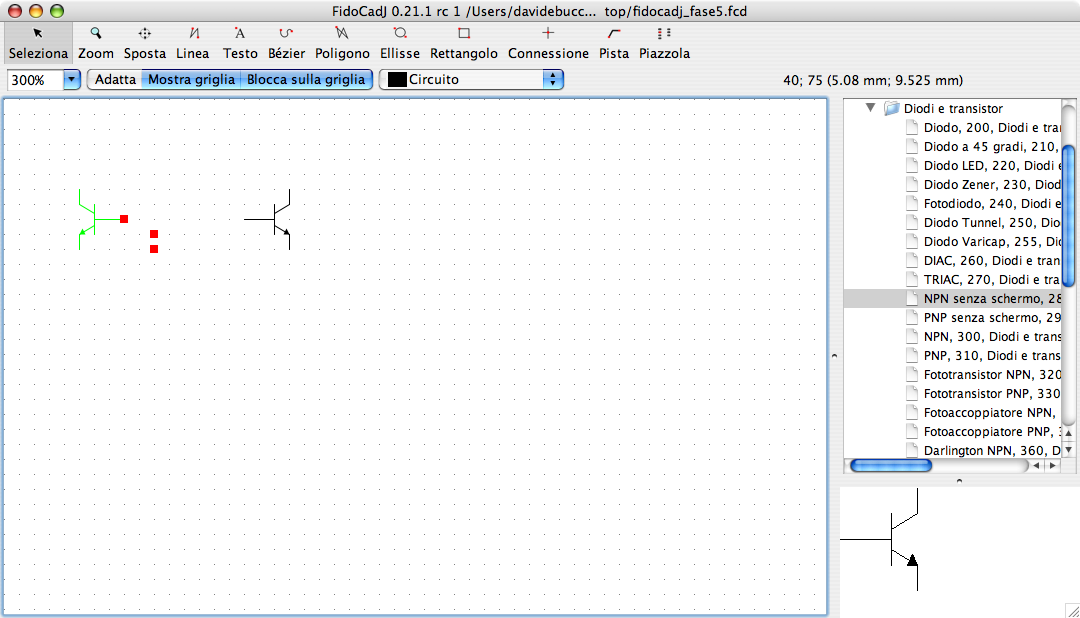
\includegraphics[width=1\textwidth,]{fidocadj_fase2} 
\caption{选择并用~\keyevidence{S}~键翻转左边的晶体管。}
\label{fig_fidocadj_fase2} 
\end{figure}

使用工具栏\index{toolbar}上的{}“直线”工具,我们可以画一些电气连接线,此时,我们意识到先前所画的元件太靠近绘图区域的边界了。这个问题很容易解决:只要选择所有已绘制的元件并移动它们到合适的位置。想要移动所有已绘制的元件,首先我们需要全部选择它们(见图~\ref{fig_fidocadj_fase3}~),选择方法:鼠标左键点击{}“选择”工具后移动到绘图区域左上角,按下鼠标左键并保持住,然后拖拉鼠标,此时会出现一个绿色矩形框(表示正在试图选择矩形范围内的所有元件),当矩形框覆盖了所有绘制元件后松开鼠标左键。现在,仍然处于选择模式,我们可以用鼠标左键点住任何一个已选择的元件后拖动所有选择的元件到所需的位置。

\begin{figure}
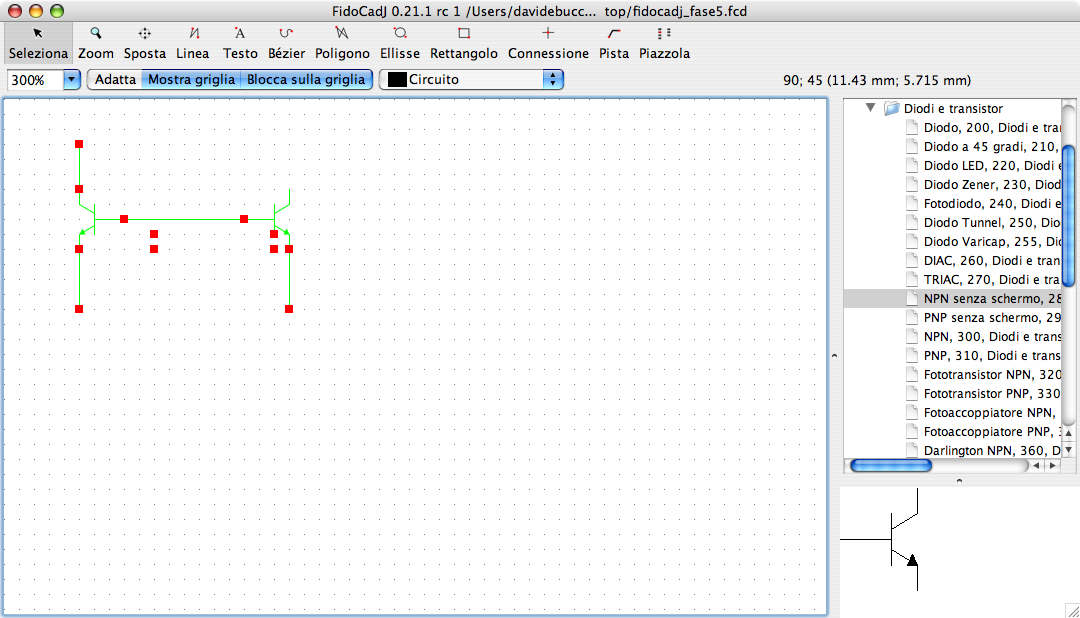
\includegraphics[width=1\textwidth,]{fidocadj_fase3} 
\caption{我们画得太靠近绘图区域上边界了:让我们选择所有已绘制的元件并把它们移动到中央。}
\label{fig_fidocadj_fase3} 
\end{figure}

然后,我们可以继续放置其它的电路图元件,如电阻\index{resistor}(Standard Library / Discrete devices / Resistor)和电源正(Standard Libreay / Basic sysbol-s / Terminal +)。我们要旋转电源正的图标,并放置到理想的位置。再次,我们可以选择它并按~\keyevidence{R}~键旋转它。到此,我们的绘图应该类似于图~\ref{fig_fidocadj_fase4}~所示的样子。

\begin{figure}
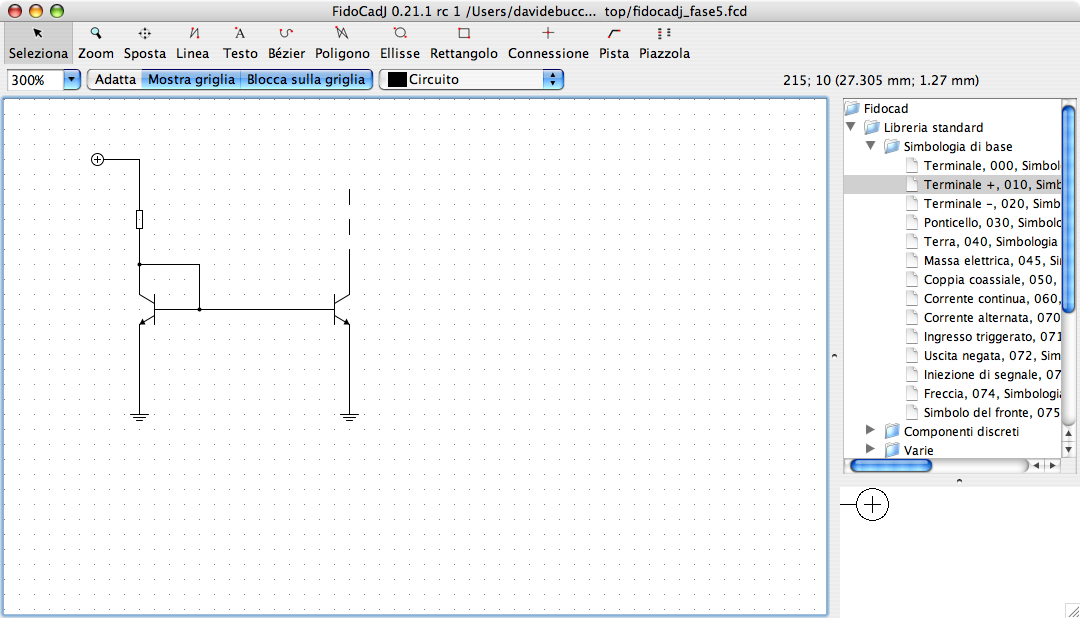
\includegraphics[width=1\textwidth,]{fidocadj_fase4} 
\caption{电路图基本完成了。}
\label{fig_fidocadj_fase4} 
\end{figure}

我们只需要加上文本和表示电流方向的箭头就能完成原理图了。在{}“Standard library / Basic symbols”中有个名称为{}“Arrow”的宏元件用于绘制箭头。我们通过左键点击工具栏上的{}“文本”\index{text}工具,并在绘图区域中想要的位置处点击来绘制文本。绘图区域中将加入一个默认的文本{}“String”,我们需要在选择模式下双击它并修改它的属性(见图~\ref{fig_param_testo}~)。晶体管(我们示例中的一对晶体管)元件的名称和编码,可以在选择模式下双击该宏元件,弹出参数窗口,其中可以设置{}“名称”和{}“编码”\footnote{允许我们对宏元件或组件符号增加名称和部件号的特性是FidoCadJ的一个扩展\index{FidoCadJ extension},这个功能在原FidoCad\index{FidoCad}中没有,见~\ref{FCJ_extension}~章节关于兼容方面的更多信息。}。建议电路原理图中的字体尺寸为垂直方向4个单位,水平方向3个单位。完成的电路原理图见图~\ref{fig_fidocadj_fase5}~。

\begin{figure}
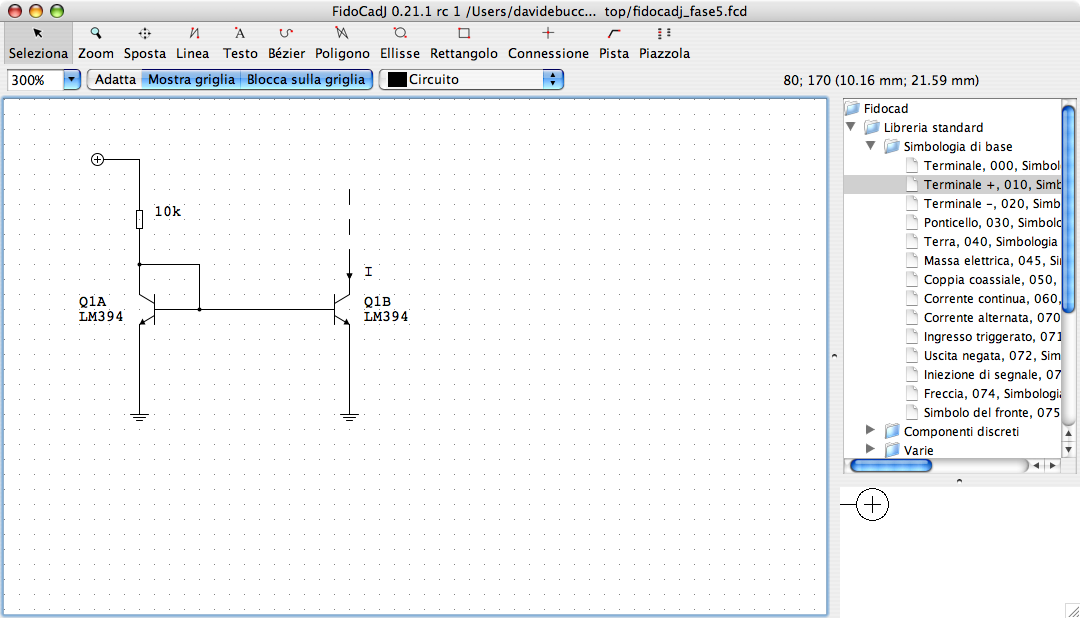
\includegraphics[width=1\textwidth,]{fidocadj_fase5} 
\caption{最终的电路图。}
\label{fig_fidocadj_fase5} 
\end{figure}

出于好奇,想知道我们示例的原理图的绘图代码\index{code}是什么样子的。只需要选择菜单{}“电路/查看绘图代码”就可以看到。现在我们可以复制原理图绘图代码并把它粘贴进电子邮件\index{e-mail}、新闻组\index{newsgroup}或论坛\index{forum}。

\begin{lstlisting}
[FIDOCAD]
MC 95 65 0 0 280
FCJ
TY 115 60 4 3 0 0 0 * Q1B
TY 115 65 4 3 0 0 0 * LM394
MC 55 65 0 1 280
FCJ
TY 20 60 4 3 0 0 0 * Q1A
TY 20 65 4 3 0 0 0 * LM394
LI 55 65 95 65 0
LI 40 75 40 95 0
LI 110 75 110 95 0
LI 40 40 40 55 0
MC 40 30 0 0 115
LI 40 15 40 30 0
LI 30 15 40 15 0
MC 30 15 2 0 010
LI 40 50 60 50 0
LI 60 50 60 65 0
SA 60 65 0
SA 40 50 0
LI 110 45 110 55 0
LI 110 35 110 40 0
LI 110 25 110 30 0
MC 40 95 0 0 040
MC 110 95 0 0 040
TY 45 30 4 3 0 0 0 * 10 k
TY 115 50 4 3 0 0 0 * I
MC 110 50 1 0 074
\end{lstlisting} 

如果您对FidoCad绘图的输出格式感兴趣,在看第~\ref{chap_formato}~章节中的详细描述。

然而,不一定要通过菜单{}“电路/查看绘图代码”复制绘图代码,我们可以选择整个绘图并拷贝(选择菜单“编辑/拷贝”或按~\keyevidence{Ctrl+C}~),然后粘贴到我们写的文本信息中,会自动以代码\index{code}的形式粘贴。

\section{层} %===================================== 2级标题

\label{sec_layer} 
用醋酸纤维薄片的概念可以帮助理解绘图中层\index{layer}的概念,先在多张醋酸纤维薄片上绘图,然后把这些醋酸纤维薄片叠加在一起组合成最终的绘图。每一层用不同的颜色绘制,且可以设置为可见或不可见。这种层的方法在许多CAD\index{CAD}软件中很常用,因为它可以简单的表示和管理叠加在一起的不同的绘图元件,比如绘制PCB\index{PCB}图就使用了层的方法。

FidoCadJ最多支持16层,层编号为0到15,并且已经指定了一些常用的层:0层为原理图层\index{electrical schematic};1层为底层导线层\index{soldering};2层为顶层导线层;3层为丝印层\index{silk-screen}。其它没有指定的层可以自由使用。通过菜单{}“视图/层”可以指定层的名称和颜色\index{colour}、设置层为可见或不可见(也即打印或不打印)。

层的顺序很重要,FidoCadJ依此绘制各层(编号相对小的层先绘制),请注意叠加层产生的覆盖作用。

\section{网格} %==================================== 2级标题

FidoCadJ绘图的逻辑单位\index{logic unit}是$5mil$($0.127mm$),不能设置半个单位。这样,任何绘图元件的坐标都是整数。这对于绘制原理图,主要是对于PCB图来说是一个非常好的分辨率\index{resolution}。然而,为了便于绘图,程序允许我们设置一个较粗糙的网格,并可以迫使鼠标放置绘图元件时对齐到最近的网格\index{grid}。有2个相关的按钮{}“显示网格”和{}“对齐到网格”。“显示网格”用于切换网格可见/不可见;“对齐到网格”用于切换鼠标放置绘图元件时需要/不需要对齐到网格。网格大小可以通过菜单“文件/选项”打开的对话框进行设置。

%======================================= 2级标题
\section{一张简单的PCB图}

实践一下目前我们所学的东西,接下来将介绍如何设计一张简单的PCB图。FidoCadJ不像其它电子CAD软件那么强大,有时侯它操作起来比较困难。FidoCadJ提供一种由原先好用的R41\index{R41 transfers}制作PCB的方法\footnote{关于R41制作PCB的方法请参考Davide Bucci的解释:\\ 
\href{http://sourceforge.net/projects/fidocadj/forums/forum/997486/topic/3923275/index/page/2}{http://sourceforge.net/projects/fidocadj/forums/forum/997486/topic/3923275/index/page/2}}转移到计算机上制作PCB的方法。很显然,在计算机上工作会具有较大的灵活性。

\marginpar{读者会发现:开发实践中,使用计算机将比使用纸和笔(以及大量的橡皮擦)得到一个清晰思路的时间要短。} 您应该知道绘制一张PCB\index{PCB}图,特别是较复杂的那种,并不是一件简单的工作。大多数CAD厂商在宣传单上注明自己的产品有自动布局\index{autoplacer}和自动布线\index{autorouter}的功能。毫无疑问,这些仍然是用户所期望的功能,发挥着重要的作用。然而,在FidoCadJ中集成的是一个非常直接和快速的绘制PCB图的方法,适用于绘制小型的可自定义尺寸的PCB图。这里,我们将介绍如何绘制一张小型的完整的PCB图。

我建议,在开始绘图前要先有一个清晰的元件布局和布线的思路,这样,可以尽可能少地避免交叉\index{crossing of tracks}。

这里我们稍微作弊一下,开始绘图前我们先看下绘图结果,见图~\ref{fig_amplificateur}~所示。这是一个简单的共射极放大器,围绕一个NPN晶体管(BC547或类似器件)建立起来的电路。可以透过元件看到PCB图,这样有助于思考实际的板子。为此,绘制元件形状的丝印层\index{silk-screen}非常有用,尽管可能对于这个DIY工程来说我们不会制作实际的板子。

\begin{figure}
\centering 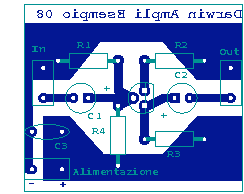
\includegraphics[width=0.5\textwidth]{amplificateur} 
\caption{一个非常简单的由NPN晶体管构成的共射极放大器电路板。}
\label{fig_amplificateur} 
\end{figure}

我建议,第一件要做的事情就是尽可能布置好所有的元件。我们的示例中有晶体管(来自元件库{}“PCB footprints / 3terminals semiconductors / TO92”),电阻(来自元件库{}“PCB footprints / Resistors / Resistor 1/4W0,4i”)和电解电容(来自元件库{}“PCB footprints / Electrolytic capacitor / Vert. diam.5mm2.5mm pitch”)。为了给出板子的边界,可以在丝印层(3层)画一个不填充的矩形。我们可以使用\emph{矩形}基元件\index{rectangle},画之前注意需要选择相应的层。到此,我们的绘图应该类似于图~\ref{fig_amplificateur_phase1}~所示的样子。\footnote{目前FidoCadJ有意大利语\index{Italian}、法语\index{French}、英语\index{English}、西班牙语\index{Spanish},德语\index{German},中文\index{Chinese}和荷兰语\index{Dutch}。翻译菜单和命令的工作很简单,如果您想FidoCadJ运行您本地语言,请通知我!也可以开展翻译库(至少是标准库)和翻译本文档的工作。}

\begin{figure}
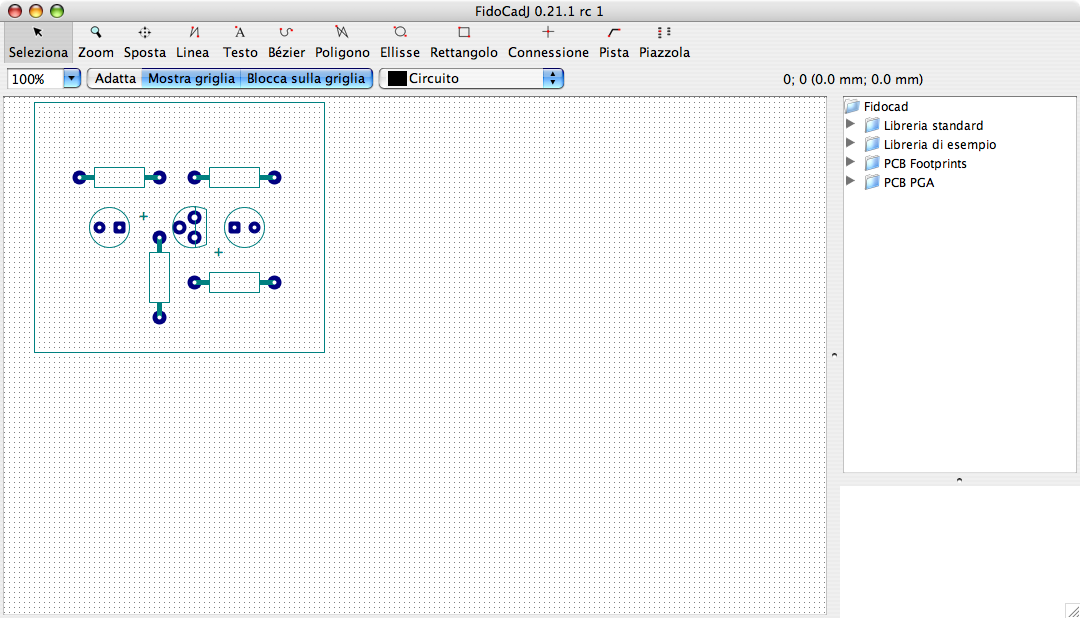
\includegraphics[width=1\textwidth]{amplificateur_phase1} 
\caption{最主要的元件已布置到板上。}
\label{fig_amplificateur_phase1} 
\end{figure}

接着我们介绍覆铜区域,电源正极和负极。它们是用多边形\index{polygon}(\emph{多边形}基元件)绘制的。在选择模式\index{selection mode}时,双击多边形边框(在弹出的对话框中)设置为填充。在绘制多边形之前,确认下当前的绘制层\index{layer}是底层导线层(1层)。电源线使用区域填充(覆铜)方式可以有效地降低寄生电感。到此,我们的绘图应该类似于图~\ref{fig_amplificateur_phase2}~所示的样子。

\begin{figure}
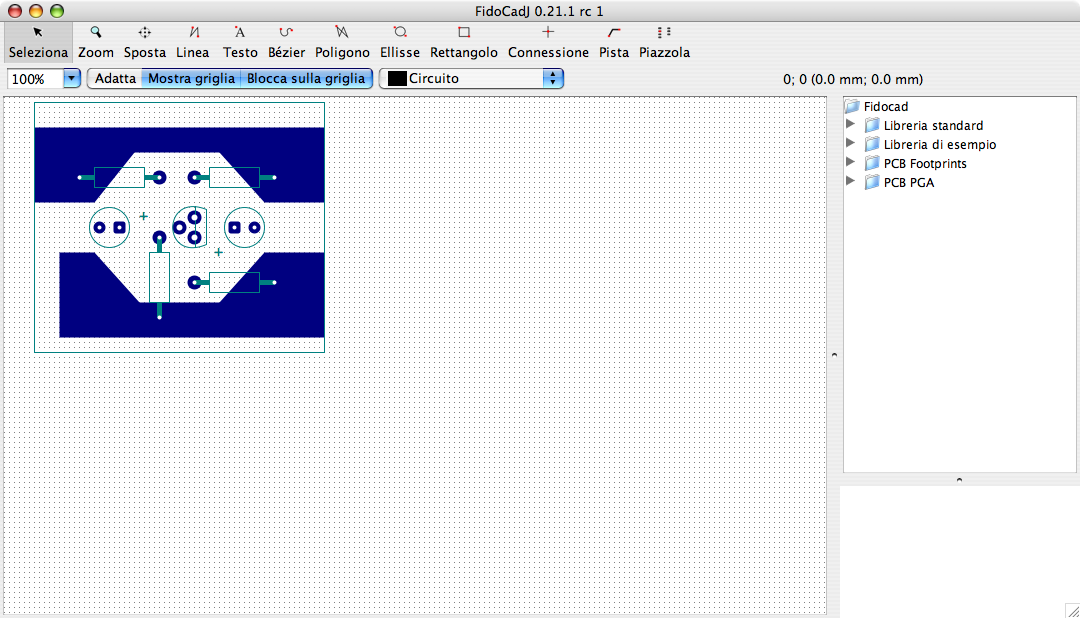
\includegraphics[width=1\textwidth]{amplificateur_phase2} 
\caption{用多边形\index{polygon}画电源线。}
\label{fig_amplificateur_phase2} 
\end{figure}

我们可以使用\emph{PCB导线}基元件\index{PCB line}来画连接导线。设置导线宽度为10个单位($1.27mm$),这样会便于焊接。 

\begin{figure}
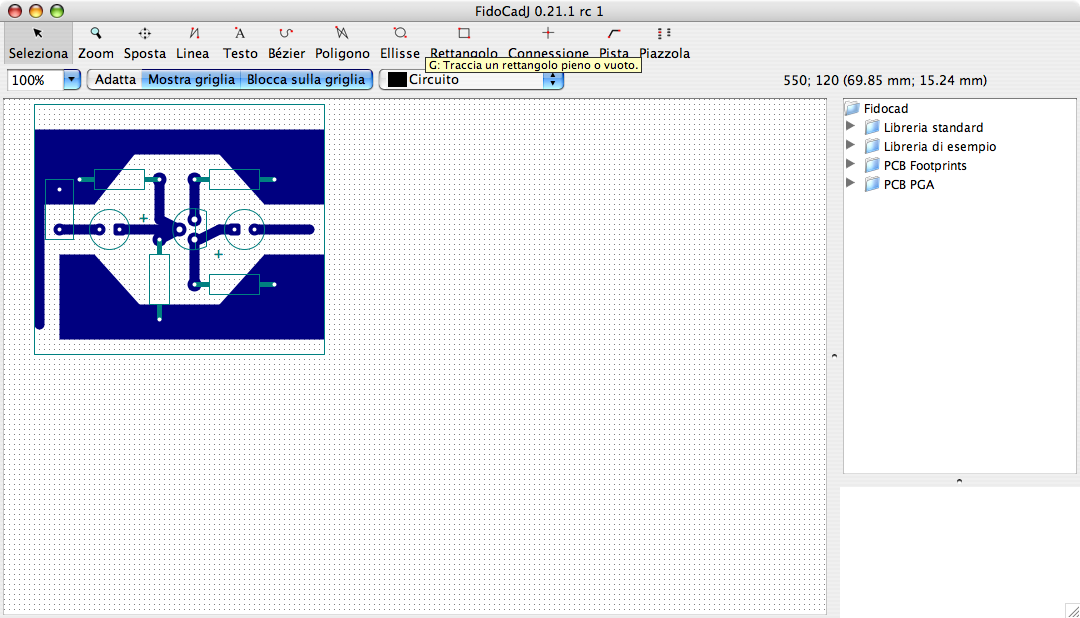
\includegraphics[width=1\textwidth]{amplificateur_phase3} 
\caption{画其它的PCB导线\index{PCB track}。}
\label{fig_amplificateur_phase3} 
\end{figure}

我们注意到还需要一些连接器:一个用于输入,一个用于输出,一个用于供电。我们使用聚酯电容类的引脚封装,其中可能有我们需要的封装规格。我们不要忘记FidoCadJ的工作思想是来自原先R41\index{R41 transfers}的制作方法。

我们可以在底层导线层(1层)放上“$+$”和“$-$”符号,在电源上并联一个陶瓷电容。\marginpar{注意导线的宽度:有时在屏幕上看起来很粗的导线实际上很细,这样的话,在焊接过程中很容易从板上脱落。}我们还可以在顶端写些文字,写在底层导线层(1层),写完后需要翻转文本\index{writings mirroring}。设置翻转很简单:切换到选择模式,双击文本弹出属性对话框,在其中设置翻转。要得到大小合适的文字需要进行一些尝试,字体的水平尺寸(宽度)和垂直尺寸(高度)的比例最好保持为3/4\index{characters dimension}。图~\ref{fig_amplificateur_phase4}~中,字体的宽度为11个单位,高度为18个单位。

\begin{figure}
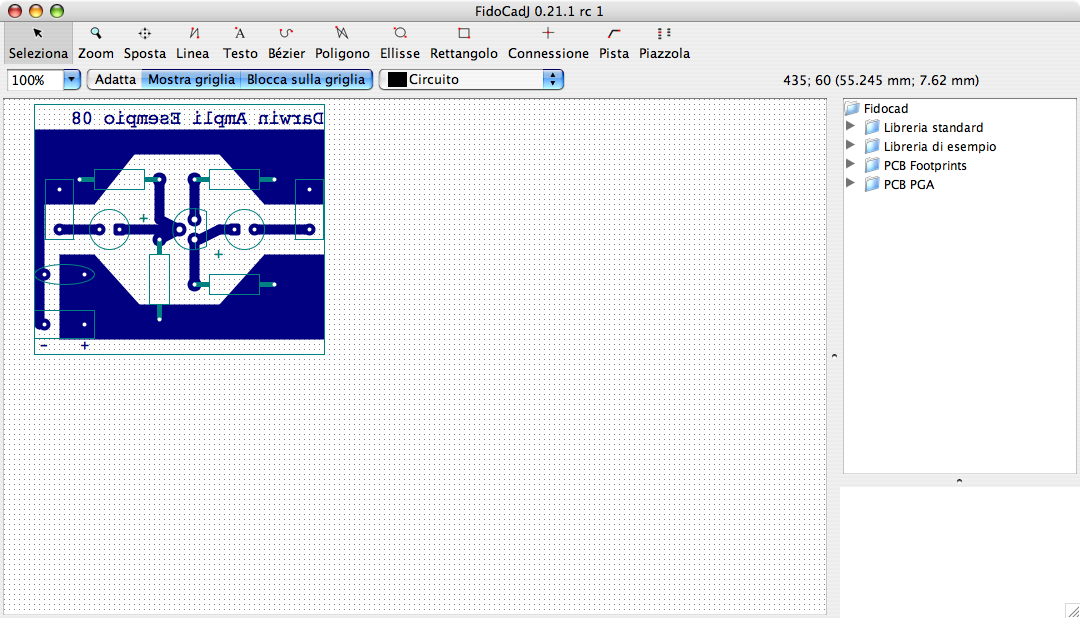
\includegraphics[width=1\textwidth]{amplificateur_phase4} 
\caption{PCB基本完成\index{PCB}。}
\label{fig_amplificateur_phase4} 
\end{figure}

目前,完成PCB图还差一件事情:为每个元件放置名称文本,这是放置在丝印层(3层)的。如图~\ref{fig_amplificateur_complet}~所示,制作完成的PCB图。

\begin{figure}
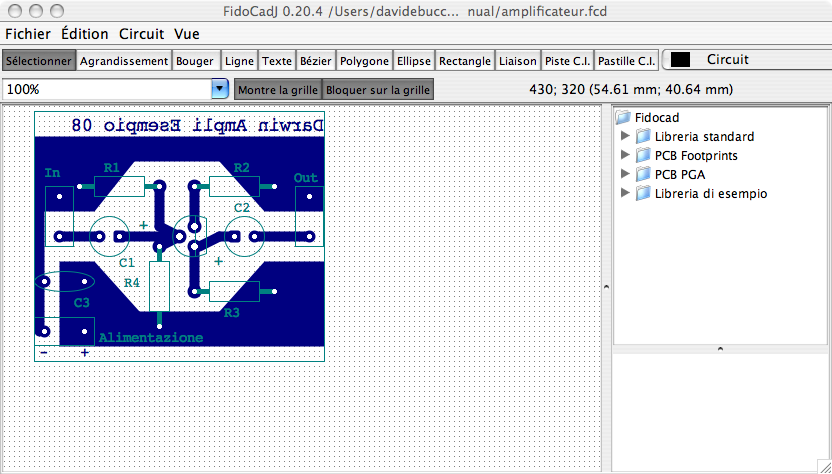
\includegraphics[width=1\textwidth]{amplificateur_complet} 
\caption{画上丝印层,工作完成。}
\label{fig_amplificateur_complet} 
\end{figure}

PCB图绘制完成后,我们可能需要打印\index{printing}它,用于制作投影机\index{printing box}使用的幻灯片,或用于其它方面(例如“Press \& Peel”\index{Press&Peel@Press\&Peel})。对于一些不需要打印的层,我们只要把它们设置成不可见就不会打印出来。可以通过菜单“视图/层”打开的对话框设置层不可见。下面的示例,我们将隐藏丝印层(3层)。应用程序将只打印底层导线层(1层)。

接着我们可以打印出屏幕上看到的所有东西(很明显,不适合纸张的大小,我们希望可以设置图纸的尺寸)。注意,选择了黑白色打印,可以得到最大的对比度。由于制造PCB\index{PCB}厂商使用的技术不同,有时可能需要翻转绘图。由于我们的PCB尺寸很小,打印出来只占了整张纸(标准ISO-UNI A4\index{A4}纸)的一个小角落,如图~\ref{fig_amplificateur_impression}~所示。

\begin{figure}
\centering \fbox{ 
\includegraphics[width=0.6\textwidth]{amplificateur_impression}} 
\caption{在ISO-UNI A4纸上(翻转)打印PCB图的效果。}
\label{fig_amplificateur_impression} 
\end{figure}

上面示例的PCB图的绘图代码信息如下(注意长的行!):

\begin{lstlisting}
[FIDOCAD]
TY 320 10 18 11 0 4 1 * Darwin Ampli Esempio 08 
TY 85 240 12 8 0 5 1 * + 
TY 44 239 12 8 0 5 1 * - 
PL 35 90 35 225 10 1
PL 55 130 95 130 10 1
PL 250 130 305 130 10 1
PL 215 130 230 130 10 1
PL 195 140 215 130 10 1
PL 115 130 175 130 10 1
MC 155 220 3 0 PCB.R01
MC 75 80 0 0 PCB.R01
MC 270 185 2 0 PCB.R01
MC 270 80 2 0 PCB.R01
MC 230 130 3 0 PCB.CE00
MC 115 130 1 0 PCB.CE00
MC 40 175 0 0 PCB.CC50
PL 190 80 190 120 10 1
PL 190 140 190 185 10 1
PL 155 80 155 120 10 1
PL 155 120 175 130 10 1
PL 155 140 175 130 10 1
PP 30 30 30 105 90 105 130 55 215 55 260 105 320 105 320 30 1
PP 320 240 320 155 260 155 215 205 135 205 90 155 55 155 55 240 1
MC 190 120 0 0 PCB.TO92
MC 305 90 1 0 PCB.CPBX352
MC 55 90 1 0 PCB.CPBX352
MC 80 225 2 0 PCB.CPBX352
TY 290 65 12 8 0 0 3 * Out 
TY 40 60 12 8 0 0 3 * In 
TY 95 225 12 8 0 0 3 * Alimentazione 
TY 70 190 12 8 0 0 3 * C3 
TY 230 95 12 8 0 0 3 * C2 
TY 115 150 12 8 0 0 3 * C1 
TY 120 170 12 8 0 0 3 * R4 
TY 220 200 12 8 0 0 3 * R3 
TY 230 55 12 8 0 0 3 * R2 
TY 100 55 12 8 0 0 3 * R1 
RV 30 5 320 255 3
\end{lstlisting} 

%======================================= 2级标题
\section{使用标尺}\index{ruler}

当绘制一张PCB图时,经常需要在图上测量尺寸。例如,你需要测下导线的宽度、两条导线之间的间隔或板卡的尺寸。FidoCadJ(从版本0.23.2开始)提供一个具有特色的标尺,让你很容易地做测量。您只需要鼠标右键点击并拖拉,就会出现一个绿色的标尺,如图~\ref{fig_fidocadj_righello}~所示。如果你的系统不支持右键点击并拖拉,你也可以在按住~\keyevidence{Shift}~键的同时用鼠标左键点击并拖拉。

\begin{figure}
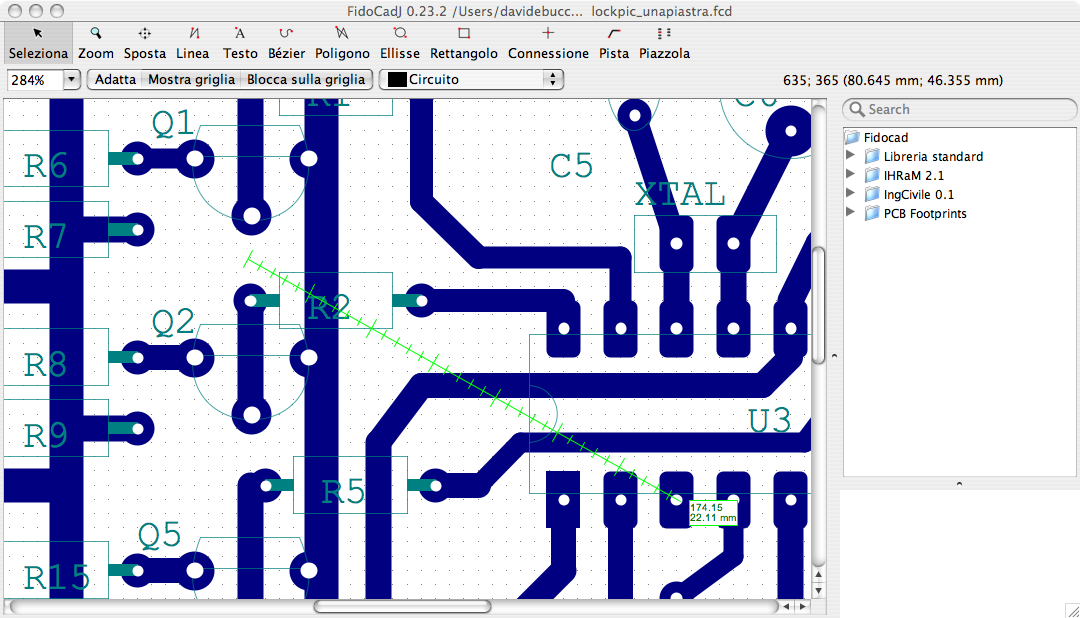
\includegraphics[width=\textwidth]{fidocadj_righello}
\caption{鼠标右键点击并拖拉,出现FidoCadJ标尺。}
\label{fig_fidocadj_righello}
\end{figure}

显示的长度值的单位是FidoCadJ的逻辑单位,另外,也有一个以毫米为单位的长度值。该功能有助于$1:1$的打印模式(例如打印PCB图)。

%======================================= 2级标题
\section{箭头和线条样式}

FicoCadJ可以设置直线、贝塞尔曲线和自然三次样条曲线的端点显示为箭头\index{arrows}。可以指定这类元件的始端或末端或两端是否显示为箭头,并且可以选择不同的箭头样式。

现在,可以选择多种线条样式\index{stroke styles},用于技术类或机械类的绘图。图~\ref{fig_gyrator}~显示了一个位于虚线框中的电路图(GIC\index{GIC})的示例。还用到一条带箭头的贝塞尔曲线。双击贝塞尔曲线,FidoCadJ显示一个参数对话框,如图~\ref{fig_parametri_bezier}~所示。你会看到选项框“始端箭头”被勾选了。FidoCadJ将根据贝塞尔曲线的绘制方向放置一个箭头。有好几种箭头样式\index{arrow styles}和线条样式\index{dashing styles}供选择,您可以尝试选择一下,了解它们之间的差别。

\begin{figure}
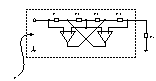
\includegraphics[width=\textwidth]{gyrator}
\caption{电路图(Antoniou通用阻抗转换器(GIC)),其中用到一些FidoCadJ的扩展。}
\label{fig_gyrator}
\end{figure}

\begin{figure}
\centering
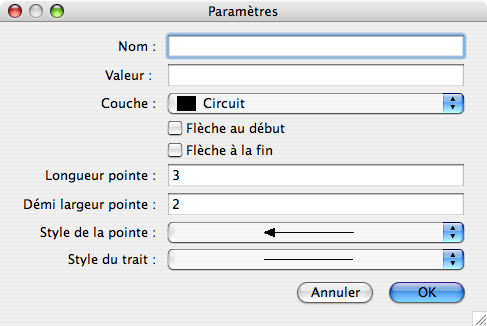
\includegraphics[width=.7\textwidth]{parametri_bezier}
\caption{图~\ref{fig_gyrator}~中的贝塞尔曲线的参数对话框。}
\label{fig_parametri_bezier}
\end{figure}

线条样式可选择和端点可显示为箭头的功能可能会与原FidoCad格式不兼容。这个意味着使用这些功能不能兼容Windows上的FidoCad\index{FidoCad}。您需要知道您使用的是FidoCadJ的扩展。如果您需要保持与FidoCad兼容,您需要通过“FidoCadJ参数设置”窗口的“FidoCadJ扩展”分页,勾上选项“完全兼容FidoCad”。通过这种方法,应用程序将不再允许你使用会引起与FidoCad兼容问题的绘图元件。如果你想要进一步了解其它绘图元件与FidoCad\index{FidoCad}的兼容性,请参考~\ref{FCJ_extension}~章节。

%======================================= 2级标题
\section{导出}

在我看来,FidoCadJ最主要的作用可能是创建用于排版的简单原理图。为此,我加入了一个重要功能——可以导出\index{exportation}多种不同文件格式的绘图。

通过菜单{}“文件/导出”即可输出当前的绘图。表~\ref{tab_esportazione}~列出了当前可以输出的图形文件格式。\marginpar{矢量格式\index{vectorial format}存储为一组绘图元件。位图格式\index{bitmap format}存储为一个像素矩阵。}表中的各种文件格式(也是FidoCadJ导出窗口中所列出的格式)都指明了它是矢量格式或位图格式。尽可能选择矢量图格式输出,这样可以获得最佳效果。\footnote{FidoCadJ结构允许加入其它文件格式,并且很方便。如果你想加入开发项目请联系我。}

导出成位图文件格式时,请选择{}“抗锯齿”,有助于减少像素化后的锯齿(对于斜线特别有效)。导出成矢量文件格式时,“分辨率”和“抗锯齿”项是无效的,此时你需要指定的是“比例”项。

{} “黑白色”项表示用纯黑色打印任何可见层。这主要用于打印准备排版或制作幻灯片使用的绘图。

\begin{table}
\centering \begin{tabular}{lp{0.7\textwidth}}
\toprule
Format  & Comment\tabularnewline
\midrule
\textsc{jpg}\index{JPG}  &  很常用的位图格式。由于它是有损压缩\index{lossy compression},不适合用于输出FidoCadJ原理图。因为常用,所以把它加了进来。\tabularnewline
\textsc{png}\index{PNG}  & 压缩的位图格式,适用于输出原理图。当不能使用矢量格式时,这可能是FidoCadJ绘图输出的最好格式。\tabularnewline
\textsc{svg}\index{SVG}  &  W3C(万维网联盟)标准矢量格式。一些因特网浏览器(例如最新版的Safari\index{Safari})可以在网页中显示它。这是个很好的图形和原理图格式,它可以使用诸如Inkscape\index{Inkscape}那样的应用程序修改FidoCadJ的绘图。目前对输出旋转和翻转的文本有些限制。\tabularnewline
\textsc{eps}\index{EPS}  &  封装的PostScript 矢量格式\index{Postscript}。对那些使用专业图形应用程序的人或那些想把FidoCadJ图纸用于\LaTeX{}\index{\LaTeX{}@\LaTeX}文档的人很有用。输出的绘图应该是完全一样的。可以用此格式输出本手册第~\pageref{fig_amplificateur}~页的图~\ref{fig_amplificateur}~所示的绘图(通过使用\textsc{pdf}~转换器,我使用的是\textsc{pdf}\LaTeX{}\index{pdf\LaTeX{}@\textsc{pdf}\LaTeX}~)。\tabularnewline
\textsc{pgf}\index{PGF}  &  在使用了CTAN的\textsl{pgf}包的\LaTeX{}\index{\LaTeX{}@\LaTeX}文档中,可以直接使用的矢量格式。该格式特别适合输出原理图,并且是一个简单的可编辑脚本。由于它的文本属性,可以直接引入到\LaTeX{}\index{\LaTeX{}@\LaTeX}代码中,本手册第~\pageref{fig_schema}~页的图~\ref{fig_schema}~示意图就使用了该技术。\tabularnewline
\textsc{scr}\index{SCR}  & FidoCadJ可以输出脚本格式的绘图,这可以被CadSoft\index{CadSoft}~的Eagle\index{Eagle}使用。使用该功能,需要在Eagle当前安装的\lstinline!lbr!库文件夹中加入\lstinline!FidoCadJLIB.lbr!库。该库可以从FicoCadJ的网站下载。在写这篇手册时,该功能还只能针对包含常见符号的原理图,有些绘图元件如焊盘和导线还不可以导出到Eagle脚本。\tabularnewline
\bottomrule
\end{tabular}
\caption{FidoCadJ输出文件格式列表。}
\label{tab_esportazione} 
\end{table}

%======================================= 2级标题
\section{命令行选项}

应用程序以\lstinline!.jar!\index{jar}格式文件发布,这是Java的档案文件\footnote{针对苹果机\index{Macintosh}发布的版本,是一个独立的应用程序。}。在多数系统上,如果机器上安装了Java\index{Java}的最新版本,只要双击文件即可运行程序。引用Sun\index{Sun}的术语,JRE\index{JRE}或Java运行环境,它是运行Java程序(不是编写Java程序,那需要SDK\dots)的必要条件也是充分条件。运行FidoCadJ至少需要Java1.5版本,这是几年前的版本了。

某些情况,需要从命令行(Unix\index{Unix}系统中的终端\index{terminal}或Windows\index{Windows}系统的MS-DOS提示符\index{MS-DOS prompt})运行FidoCadJ。这时,只需要运行带\lstinline!-jar!选项的\lstinline!java!命令:

\begin{lstlisting} 
java -jar fidocadj.jar
\end{lstlisting}

如果命令行\index{command line}中同时指定一个需要打开的绘图文件,FidoCadJ将运行并试着打开它,例如(在Unix\index{Unix}机器上):

\begin{lstlisting} 
java -jar fidocadj.jar ~/FidoCadJ/test.fcd 
\end{lstlisting}

FidoCadJ将运行并试着打开文件\lstinline!~/FidoCadJ/test.fcd!(假如该文件存在)。

FidoCadJ还能做其它有趣的事情,选项\lstinline!-h!查看FidoCadJ的选项信息:
\lstset{basicstyle=\scriptsize\ttfamily}
	 	 
\begin{lstlisting}
[davidebucci@Darwin]$ java -jar fidocadj.jar -h

This is FidoCadJ, version 0.24.1.
By Davide Bucci, 2007-2012.

Use: java -jar fidocadj.jar [-options] [file] 
where options include:

 -n     Do not start the graphical user interface (headless mode)

 -d     Set the extern library directory
        Usage: -d dir
        where 'dir' is the path of the directory you want to use.

 -c     Convert the given file to a graphical format.
        Usage: -c sx sy eps|pdf|svg|png|jpg|fcd|sch outfile
        If you use this command line option, you *must* specify a FidoCadJ
        file to convert.
        An alternative is to specify the resolution in pixels per logical unit
        by preceding it by the letter 'r' (without spaces), instead of giving
        sx and sy.

 -s     Print the size  of the specified file in logical coordinates.

 -h     Print this help and exit.

 -t     Print the time used by FidoCadJ for the specified operation.

 -p     Do not activate some platform-dependent optimizations. You might try
        this option if FidoCadJ hangs or is painfully slow.

 -l     Force FidoCadJ to use a certain locale (the code might follow
        immediately or be separated by an optional space).

 [file] The optional (except if you use the -d or -s options) FidoCadJ file to
        load at startup time.

Example: load and convert a FidoCadJ drawing to a 800x600 pixel png file
        without using the GUI.
  java -jar fidocadj.jar -n -c 800 600 png out1.png test1.fcd

Example: load and convert a FidoCadJ drawing to a png file without using the
        graphic user interface (the so called headless mode).
        Each FidoCadJ logical unit will be converted in 2 pixels on the image.
  java -jar fidocadj.jar -n -c r2 png out2.png test2.fcd

Example: load FidoCadJ forcing the locale to simplified chinese (zh).
  java -jar fidocadj.jar -l zh


[davidebucci@Darwin]$
\end{lstlisting}
\lstset{language=FIDOCAD,
    basicstyle=\small\ttfamily}
    
最简单的选项\lstinline!-n!,软件运行\dots\ 不出现GUI。这个选项,是把Java的环境变量\lstinline!java.awt.headless!设置为true。显然,单独使用该选项没什么意义,需要和其它的选项组合使用。选项\lstinline!-d!指定FidoCadJ在启动时加载库的文件夹。选项\lstinline!-c!允许你使用FidoCadJ把FidoCad文件(必须指定)转换成一张矢量或位图格式的图片,这时把FidoCadJ当作转换器使用,并不需要GUI交互(与\lstinline!-n!选项一起使用)。

看我们的第一个示例,可以帮助我们理解:
	 	
\begin{lstlisting}
java -jar fidocadj.jar -n -c 800 600 png out1.png test1.fcd
\end{lstlisting}

FidoCadJ将运行但不激活GUI,并从\lstinline!test1.fcd!文件导出png\index{PNG}格式的文件。导出文件名称为\lstinline!out1.png!,像素大小为800*600。\lstinline!-c!选项还有另一种参数——指定转换时一个逻辑单位对应多少个像素(假定该参数为$r_\mathrm{p}$)。FidoCadJ不能处理半像素(指定的必须为整数),经过实践,认为设置$r_\mathrm{p}$为2,即1个逻辑单位对应2个像素,可以保证原理图总是能看得清楚(尽管可能有点小)。参数$r_\mathrm{p}$可以为非整数,见以下示例:

\begin{lstlisting}
java -jar fidocadj.jar -n -c r1.25 png out2.png test2.fcd
\end{lstlisting}

要知道原理图的总大小(逻辑单位),你可以使用\lstinline!-s!选项。记住,不管哪种方式,转换时FidoCadJ总是在电路图的边缘加入$t_\mathrm{margin}=3$个逻辑单位。因此,假定$t_\mathrm{w}$为绘图的逻辑单位数(通过\lstinline!-s!选项查看),导出绘图的像素数$p_\mathrm{w}$的计算公式如下:

\begin{equation}
p_\mathrm{w} = r_\mathrm{p} (t_\mathrm{w}+ 2 t_\mathrm{margin})
\end{equation}

另一个有趣的选项(该特性主要来自Java\index{Java}而非FidoCadJ)就是可以修改应用程序的外观(Java称之为LookAndFeel\index{look  feel@look \& feel})。你可以选择你喜欢的LookAndFeel,而不需要修改一行代码。这里有个Linux\index{Linux}用户使用的外观GTK+\index{GTK+} LookAndFeel。
\begin{lstlisting} 
java -Dswing.defaultlaf=com.sun.java.swing.plaf.gtk.GTKLookAndFeel -jar fidocadj.jar 
\end{lstlisting} 
还有个经典的Motif\index{Motif} LookAndFeel,如图~\ref{fig_fidocadj_motif}所示\footnote{MacOSX上的这种风格可能会令那些熟悉非常优雅的图形接口的用户感到莫名其妙得吃惊,例如Aqua。而几年前我看到的基于Motif的图形界面上的同步控制系统,也是异常的漂亮!}。
\begin{lstlisting}
java -Dswing.defaultlaf=com.sun.java.swing.plaf.motif.MotifLookAndFeel -jar fidocadj.jar 
\end{lstlisting} %
\begin{figure}
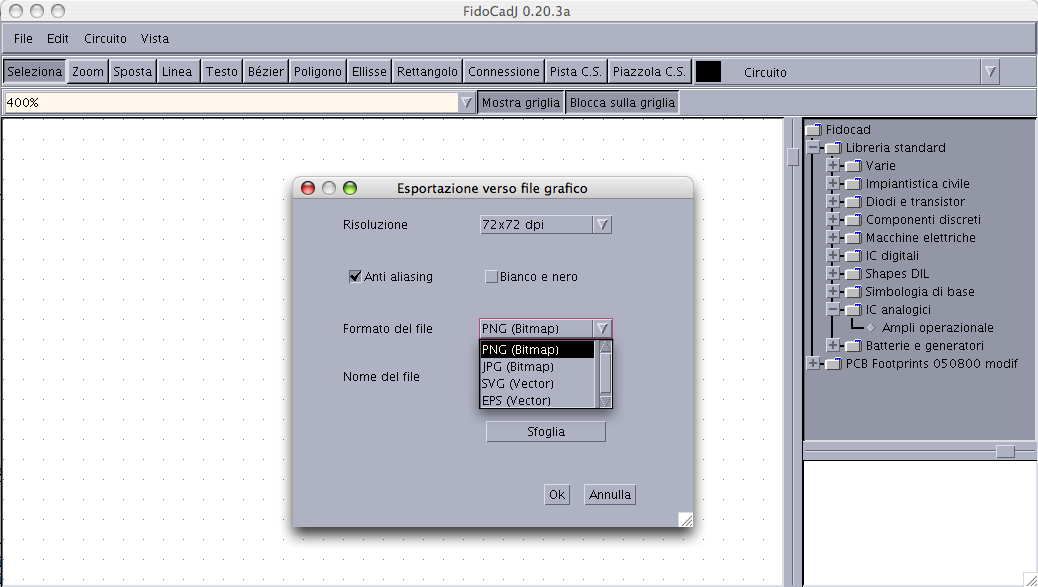
\includegraphics[width=1\textwidth]{fidocadj_motif} 

\caption{在MaxOSX\index{MacOSX}上程序的外观,使用Motif LookAndFeel。}

\label{fig_fidocadj_motif} 
\end{figure}


很明显,上面列出的命令需要在终端中输入,确保当前目录中包含文件\lstinline!fidocad.jar!,并在同一行中输入。

\lstset{language=FIDOCAD,
 basicstyle=\small\ttfamily}

%======================================= 2级标题
\section{库管理}

应用程序允许我们指定加载库\index{library}文件(扩展名为\lstinline!.fcl!的文件)的目录。可以通过菜单{}“文件/选项”进行设置。如果目录中存在一个\lstinline!FCDstdlib.fcl!库文件,加载这个库文件将取代应用程序中的标准库\index{library!standard library}。类似的,如果存在一个\lstinline!PCB.fcl!库文件,将取代PCB库\footnote{注意使用大写字母,特别是你的系统的文件管理是区分字母大小写的。}。其它扩展名为\lstinline!.fcl!的库文件,被认为是增加的库,会和标准库一起加载。感谢Roby IZ1CYN的付出,从0.23版开始,我可以直接在FidoCadJ发行版内部包含IHRaM 3.1库\index{IHRaM library}。之所以包含这个库,是因为目前为止它是我见过的所有库中内容最完整、结构最合理的一个库。由于这个库已经是FidoCadJ的嵌入库,如果当前加载库路径中包含\lstinline!IHRAM.FCL!库文件,这个库将被认为是增加的库被加载到程序中并显示版本号。你也可以增加文件名为\lstinline!elettrotecnica.fcl!的电气符号库。

加载库搜索路径中的其它一些扩展名为\lstinline!.fcl!的文件将被认为是库文件。当用户改变了库加载路径,需要选择菜单“电路/更新库”。

从版本0.23开始,FidoCadJ可以拆分非标宏元件(拆分成原FidoCad\index{FidoCad}可以识别的元件)。这个功能对于在新闻组中粘贴绘图很有用,因为该功能可以把每个不是标准FidoCad\index{FidoCad}库的宏元件拆分为FidoCad可识别元件。这样,看你的帖子并不需要和你安装同样的库。激活该功能,选择菜单“文件/选项”,在“FidoCadJ扩展”分页上可以勾选拆分非标准宏元件的选项,这里可以选择在保存文件时 和/或 复制/粘贴(部分或全部)绘图时激活这个动作。

\chapter{绘图格式、宏元件和库} \label{chap_formato}

本章详细描述FidoCad绘图格式,即FidoCadJ基本绘图格式。这是一种简单的文本格式,其优点是紧凑且高效。目前为止,还没有详细描述该格式的文档,这里我只是努力把全部所知道的总结出来。另外,我对FidoCad绘图格式做了一些扩展(仅适用于FidoCadJ),称之为FidoCadJ扩展绘图格式,本章也描述了这些扩展绘图格式。请记住,FidoCadJ(从0.23.4版本开始)的绘图文件在任何平台上只使用UTF-8\index{UTF-8}编码格式\index{encoding}\footnote{注意绘图格式与编码格式的区别:绘图格式是描述图形使用的文本的格式;编码格式是描述文件的计算机存储的格式,这里UTF-8编码格式为存储FidoCadJ绘图文件的计算机存储的格式。 }。

%======================================= 2级标题
\section{绘图文件头}

所有FidoCad\emph{\index{FidoCad}}的绘图文件,都必须以\emph{\lstinline!{[}FIDOCAD{]}!}标记开头。程序通过此标记才能识别出是FidoCad\emph{\index{FidoCad}}的绘图文件,然后才开始解析其中的命令行。在这点上,FidoCadJ要比FidoCad宽松,没有以该标记开头\emph{\index{header}}的绘图文件也可以得到解析,并且会跳过错误的命令行,但错误命令行的数量不能超过程序内部设置的一个值(大约100行),这确保FidoCadJ在打开它不能解析的文件时不会浪费过多的时间。

%======================================= 2级标题
\section{坐标系统}

FidoCadJ绘图的坐标系统\emph{\index{coordinates system}}非常简单。事实上,它是一个非常大的正向坐标区域。X向和Y向的单位长度都固定为\emph{$5mil$}(\emph{$0.127mm$}),这个单位长度对于显示最小的SMD封装器件来说,它也是一个很好的分辨率,日常应用已经足够了。打印时,FidoCadJ绘图的分辨率是每英寸200点。

原FidoCad\emph{\index{FidoCad}}有两种不同的绘图模式:绘制PCB图\emph{\index{PCB}}模式和绘制电路原理图\index{electrical schematic}模式。在FidoCadJ中,这两种绘图模式已经不加以区分了,只是在打印绘图时才区别对待。因为,由程序来调整绘制的电路原理图打印比例,使之适合打印纸张是非常合理的,不然,打印出来的电路原理图有可能只有邮票那么大。

%======================================= 2级标题
\section{绘图元件}

\label{sec_primitive}
FidoCadJ有12种绘图元件,列出如下:
\begin{itemize}
\item 直线\index{line}
\item 填充或不填充的矩形\index{rectangle} 
\item 简单文本(已废弃)
\item 高级文本\index{text}
\item 填充或不填充的多边形\index{polyline}
\item 填充或不填充的椭圆形\index{ellipse} 
\item 贝塞尔曲线\index{B�zier} 
\item 自然三次样条曲线\index{spline}
\item 电气连接点\index{connection}
\item PCB焊盘\index{PCB pad}
\item PCB导线\index{PCB track}
\item 宏元件\index{macro}
\end{itemize}

下面我们将逐一讲解它们。各种绘图元件\index{element}有相应的带参数\index{parameters}的命令定义。通常情况是,一条命令行对应一个绘图元件,命令行中有命令和参数(一般为整数数字或文本字符串),命令和参数/参数和参数之间用空格隔开。

%======================================= 4级标题
\subsubsection{直线}

直线\index{line}\marginpar{数学家们可能认为描述为“线段”\index{segment}更合适。}由\lstinline!LI!\index{LI}命令定义,其命令参数有:起点坐标、终点坐标、层号。

\begin{lstlisting}
LI x1 y1 x2 y2 l 
\end{lstlisting} 
其中,$(x_{1},y_{1})$和$(x_{2},y_{2})$分别表示起点坐标和终点坐标;$l$表示层号(整数,取值范围为[0,15])。

\textbf{FidoCadJ扩展}: 从0.23版本开始,可以在\lstinline!LI!\index{LI}命令后紧跟一条扩展命令:
\begin{lstlisting} 
FCJ a b c d e nv
\end{lstlisting}
其中,$a$表示端点形状(取值及含义请见表~\ref{tab_frecce_estremita});$b$表示端点箭头样式(取值及含义请见表~\ref{tab_frecce_stile});$c$和$d$分别表示箭头长度和箭头宽度的一半;$e$表示线条样式(整数);$nv$等于1则\lstinline!FCJ!命令后紧跟2条\lstinline!TY!命令,给出该元件关联的名称和编码,等于0则没有。

\begin{table}
\centering

\begin{tabular}{ccp{.7\textwidth}}
\toprule
$a$	& 端点形状 \\
\midrule
0	& 无箭头 \\
1	& 始端箭头\\
2	& 末端箭头\\
3	& 两端箭头\\
\bottomrule
\end{tabular}
\caption{表示线条类基元件的端点箭头的$a$参数的含义。}
\label{tab_frecce_estremita}
\end{table}

\begin{table}
\centering
\begin{tabular}{ccp{.7\textwidth}}
\toprule
$b$	& 端点箭头样式 \\
\midrule
0	& 标准箭头 \\
1	& 标注标准箭头 \\
2	& 空心箭头\\
3	& 标注空心箭头\\
\bottomrule
\end{tabular}
\caption{表示箭头样式的$b$参数的含义。}
\label{tab_frecce_stile}
\end{table}

%======================================= 4级标题
\subsubsection{填充或不填充的矩形}

填充或不填充的矩形\index{rectangle}由\lstinline!RP!\index{RP}和\lstinline!RV!\index{RV}命令定义,其命令参数有:矩形的任意一条对角线的2个顶点坐标、层号。
\begin{lstlisting} 
RP x1 y1 x2 y2 l 
RV x1 y1 x2 y2 l 
\end{lstlisting}
其中,$(x_{1},y_{1})$和$(x_{2},y_{2})$分别表示矩形对角线的2个顶点坐标;$l$表示层号(整数,取值范围为[0,15])。

\textbf{FidoCadJ扩展}: 从0.23版本开始,可以在\lstinline!RP!\index{RP}或\lstinline!RV!\index{RV}命令后紧跟一条扩展命令:
\begin{lstlisting} 
FCJ e nv
\end{lstlisting}
其中,$e$表示线条样式(整数)。$nv$等于1则\lstinline!FCJ!命令后紧跟2条\lstinline!TY!命令,给出该元件关联的名称和编码,等于0则没有。 

%======================================= 4级标题
\subsubsection{简单文本(已废弃)}

简单文本\index{simple text}是FidoCad\index{FidoCad}早期版本中使用的文本元件。FidoCadJ把它解析为12个单位的大小固定的文本,不随绘图缩放\index{zoom}而变化。

由于FidoCad的创建者Lorenzo Lutti\index{Lorenzo Lutti}认为该元件已经淘汰,并把它废弃掉了\index{obsolete},FidoCadJ采取了同样的做法。然而,为了能够正确解析旧文件,FidoCadJ还是能够识别它,但当保存文件时,将使用\lstinline!TY!\index{TY}命令存储该元件(转化为高级文本)。

简单文本由\lstinline!TE!\index{TE}命令定义,格式如下:
\begin{lstlisting} 
TE x1 y1 �text to be written 
\end{lstlisting}
其中,$(x_{1},y_{1})$是文本的位置坐标;“text to be written”表示实际的文本内容。注意没有层信息。FidoCadJ默认该元件在0层(原理图层\index{circuit})。

%======================================= 4级标题
\subsubsection{高级文本}

相比上面介绍的简单文本\index{simple text},高级文本\index{advanced text}的功能更加丰富。

高级文本由\lstinline!TY!\index{TY}命令定义,其命令参数有:文本位置坐标、文本高度、文本宽度、文本样式、层号、字体和文本。由于信息量比较多,这条命令有点复杂。
\begin{lstlisting}
TY x1 y1 sy sx a s l f �text to be written 
\end{lstlisting}
其中,$(x_{1},y_{1})$表示文本的位置坐标;$s_{y}$和$s_{x}$分别表示文本使用字体的高度和宽度(逻辑单位\index{logical unit}数。我通常先设置字体高度,再根据字体高度设置字体宽度,这样的话需要有一个确定的斜率);$a$表示文本旋转(以1/60度为旋转单位);$s$表示文本样式\index{text!style}(见表~\ref{tab_stile_testo});$l$表示层号(整数,取值范围为[0,15]);$f$表示字体名称(如果字体名称包含空格,需要把空格替换成+号\index{+};或可以用星号\index{asterisk},表示使用标准的Courier New字体\index{Courier New});“text to be written”表示实际的文本内容。

\begin{table}
\centering \begin{tabular}{llp{0.7\textwidth}}
\toprule 位  & 位值  & 动作 \tabularnewline
\midrule 0  &  1  &  加粗\tabularnewline
1  & 2  &  倾斜\tabularnewline
2  & 4  &  翻转文本\tabularnewline
\bottomrule % &  & \tabularnewline
\end{tabular}
\caption{文本样式字段位的含义。}
\label{tab_stile_testo} 
\end{table}

文本\index{maximum length of text}的最大长度为80个单词。这里以单词为计数对象,而不是字符,是因为在国际化程序中,是把命令行分解成单词进行解析的。

%======================================= 4级标题
\subsubsection{填充或不填充的多边形}

填充的或不填充的多边形\index{poliline}由\lstinline!PP!\index{PP}和\lstinline!PV!\index{PV}命令定义,其命令参数有:多边形的各顶点坐标、层号。
\begin{lstlisting}
PP x1 y1 x2 y2 ... l 
PV x1 y1 x2 y2 ... l 
\end{lstlisting} 
其中,$(x_{1},y_{1})$,$(x_{2},y_{2})$\dots\ 表示多边形的各顶点坐标;$l$表示层号(整数,取值范围为[0,15])。顶点个数越多命令行越长,为避免命令行过长,顶点个数最多为20个\index{maximum number of vertices}。

\textbf{FidoCadJ扩展}: 从0.23版本开始,可以在\lstinline!PP!\index{PP}和\lstinline!PV!\index{PV}命令后紧跟一条扩展命令::
\begin{lstlisting} 
FCJ e nv
\end{lstlisting}
其中,$e$表示线条样式(整数);$nv$等于1则\lstinline!FCJ!命令后紧跟2条\lstinline!TY!命令,给出该元件关联的名称和编码,等于0则没有。

%======================================= 4级标题
\subsubsection{填充或不填充的椭圆}

填充或不填充的椭圆\index{ellipse}由\lstinline!EP!\index{EP}和\lstinline!EV!\index{EV}命令定义,其命令参数有:椭圆外接矩形的任意一条对角线的2个顶点的坐标、层号。
\begin{lstlisting} 
EP x1 y1 x2 y2 l 
EV x1 y1 x2 y2 l 
\end{lstlisting} 
其中,$(x_{1},y_{1})$和$(x_{2},y_{2})$表示椭圆外接矩形的对角线的2个顶点;$l$表示层号(整数,取值范围为[0,15])。

\textbf{FidoCadJ扩展}: 从0.23版本开始,可以在\lstinline!EP!\index{EP}和\lstinline!EV!\index{EV}命令后紧跟一条扩展命令:
\begin{lstlisting} 
FCJ e nv
\end{lstlisting}
其中,$e$表示线条样式(整数);$nv$等于1则\lstinline!FCJ!命令后紧跟2条\lstinline!TY!命令,给出该元件关联的名称和编码,等于0则没有。

%======================================= 4级标题
\subsubsection{贝塞尔曲线}

贝塞尔\index{B�zier}曲线,是使用3次方程,由4个顶点控制的曲线。它由\lstinline!BE!\index{BE}命令定义,其命令参数有:各控制点坐标、层号。
\begin{lstlisting} 
BE x1 y1 x2 y2 x3 y3 x4 y4 l 
\end{lstlisting} 
其中,$P_{1}\equiv(x_{1},y_{1})$, $P_{2}\equiv(x_{2},y_{2})$, $P_{3}\equiv(x_{3},y_{3})$, $P_{4}\equiv(x_{4},y_{4})$这4个贝塞尔\index{B�zier}曲线的控制点,$l$表示层号(整数,取值范围为[0,15])。上面给予的4个顶点,曲线可以通过下面表达式计算。\begin{equation}
B(t)=(1-t)^{3}P_{1}+3t(1-t)^{2}P_{2}+3t^{2}(1-t)P_{3}+t^{3}P_{4},\end{equation}
其中$t\in[0,1]$,是一个参数。

\textbf{FidoCadJ扩展}: 从0.23版本开始,可以在\lstinline!BE!\index{BE}命令后紧跟一条扩展命令:
\begin{lstlisting} 
FCJ a b c d e nv
\end{lstlisting}
其中,$a$表示端点形状(取值及含义请见表~\ref{tab_frecce_estremita});$b$表示端点箭头样式(取值及含义请见表~\ref{tab_frecce_stile});$c$和$d$分别表示箭头长度和箭头宽度的一半;$e$表示线条样式(整数);$nv$等于1则\lstinline!FCJ!命令后紧跟2条\lstinline!TY!命令,给出该元件关联的名称和编码,等于0则没有。

%======================================= 4级标题
\subsubsection{自然三次样条曲线(复杂曲线)}
自然三次样条曲线\index{spline},是由一些顶点控制的曲线,该曲线以一种平滑的计算方式经过每个顶点\footnote{ \href{http://www.cse.unsw.edu.au/~lambert/splines/natcubic.html}{http://www.cse.unsw.edu.au/\textasciitilde lambert/splines/natcubic.html}}。它由\lstinline!CV!\index{CV}和\lstinline!CP!\index{CP}命令定义,其命令参数有:各控制点坐标、层号。
\begin{lstlisting}
CV aa x1 y1 x2 y2 ... l
CP aa x1 y1 x2 y2 ... l
\end{lstlisting}
其中,$aa$等于1则曲线闭合,等于0则曲线开放;$(x_1, y_1)$,$(x_2, y_2)$\dots\ 表示各控制点坐标;$l$表示层号(整数,取值范围为[0,15])。同矩形类似,顶点个数越多命令行越长,为避免命令行过长,顶点个数最多为100个\index{maximum number of vertices}。命令行长度取决于顶点的数量。该元件在0.24版本中引入,原FidoCAD\index{FidoCAD}中没有。

\textbf{FidoCadJ扩展}: 可以在\lstinline!CV!\index{CV}和\lstinline!CP!\index{CP}命令后紧跟一条扩展命令:
\begin{lstlisting} 
FCJ a b c d e nv
\end{lstlisting}
其中,$a$表示端点形状(取值及含义请见表~\ref{tab_frecce_estremita});$b$表示端点箭头样式(取值及含义请见表~\ref{tab_frecce_stile});$c$和$d$分别表示箭头长度和箭头宽度的一半;$e$表示线条样式(整数);$nv$等于1则\lstinline!FCJ!命令后紧跟2条\lstinline!TY!命令,给出该元件关联的名称和编码,等于0则没有。

%======================================= 4级标题
\subsubsection{电气连接点}
电气连接点\index{junction}是一个很简单的填充的圆形,尺寸固定(圆形的直径在程序中设置为2个逻辑单位),用于表示电路原理图中的电气连接。由\lstinline!SA!\index{SA}命令定义,其命令参数有:位置坐标、层:
\begin{lstlisting}
SA x1 y1 l 
\end{lstlisting} 

\textbf{FidoCadJ扩展}: 可以在\lstinline!SA!\index{SA}命令后紧跟扩展命令\lstinline!FCJ!,\lstinline!FCJ!命令后紧跟2条\lstinline!TY!命令,给出该元件关联的名称和编码。

%======================================= 4级标题
\subsubsection{PCB焊盘}

PCB焊盘\index{PCB pad}由\lstinline!PA!\index{PA}命令定义,其命令参数有:样式(椭圆形,矩形,圆角矩形)、内部孔的直径。
\begin{lstlisting}
PA x1 y1 dx dy si st l 
\end{lstlisting} 
其中,$(x_{1},y_{1})$表示焊盘的位置坐标;$d_{x}$表示焊盘的宽度(也就是焊盘$x$向的尺寸);$d_{y}$表示焊盘的高度(也就是焊盘$y$向的尺寸);$s_{i}$表示焊盘过孔的直径,$s_{t}$表示焊盘的样式:
\begin{itemize}
\item [0] 椭圆形焊盘
\item [1] 矩形焊盘
\item [2] 圆角矩形焊盘
\end{itemize}
$l$表示层号(整数,取值范围为[0,15])。

\textbf{FidoCadJ扩展}: 可以在\lstinline!PA!\index{PA}命令后紧跟扩展命令\lstinline!FCJ!,\lstinline!FCJ!命令后紧跟2条\lstinline!TY!命令,给出该元件关联的名称和编码。

%======================================= 4级标题
\subsubsection{PCB导线}

PCB导线\index{PCB track}是可以指定宽度的线段,线段两端总是圆的,便于连接其它PCB导线或焊盘。它由\lstinline!PL!\index{PL}命令定义,其命令参数有:起点坐标、终点坐标、宽度、层号。
\begin{lstlisting} 
PL x1 y1 x2 y2 di l 
\end{lstlisting}
其中,$(x_{1},y_{1})$和$(x_{2},y_{2})$分别表示起点坐标和终点坐标;$d_{i}$表示宽度;$l$表示层号(整数,取值范围为[0,15])。

\textbf{FidoCadJ扩展}: 可以在\lstinline!PL!\index{PL}命令后紧跟扩展命令\lstinline!FCJ!,\lstinline!FCJ!命令后紧跟2条\lstinline!TY!命令,给出该元件关联的名称和编码。

%======================================= 4级标题
\subsubsection{宏元件}

宏元件\index{macro}是一个库中的符号,也可以说是一个绘图。通常,电气符号就采用这种表示方法。它由\lstinline!MC!\index{MC}命令调用一个宏,命令参数有:调用如下:
\begin{lstlisting} 
MC x1 y1 o m n 
\end{lstlisting} 
其中,$(x_{1},y_{1})$表示宏元件的位置坐标;$o$表示宏元件的方向(方向值乘以90\textdegree{}的顺时针方向);$m$等于1则宏元件翻转;$n$表示宏元件在库中的名称,作为特定的\emph{库中的代号}。

如果\lstinline!MC!\index{MC}命令后跟着\lstinline!FCJ!命令,\lstinline!FCJ!命令后面需要跟2个\lstinline!TY!命令,指定该元件的名称和编号。

%======================================= 2级标题
\section{FidoCadJ扩展}
\label{FCJ_extension}

从0.21版本开始,FidoCadJ在原FidoCad格式\index{FidoCadJ extension}的基础上引入了一些好的改进,称为FidoCadJ扩展。绘图代码中用\lstinline!FCJ!\index{FCJ}命令表示进行FidoCadJ扩展。该命令单独使用没有意义,而是用于表明FidoCadJ需要对前一行中定义的东西给出更多的信息。这里有个示例:
\begin{lstlisting}
[FIDOCAD]
MC 40 30 0 0 080
FCJ
TY 50 35 4 3 0 0 0 * R1
TY 50 40 4 3 0 0 0 * 47k
\end{lstlisting}
在\lstinline!MC!命令后紧跟1条\lstinline!FCJ!命令,表示将对\lstinline!MC!命令定义进行扩展,扩展定义为紧跟的2条\lstinline!TY!命令,定义出关联的名称和编码。

FidoCadJ可以通过设置选项“完全兼容FidoCad”禁用所有的扩展,这样,FidoCadJ完全兼容原FidoCad\index{FidoCad}。然而,FidoCadJ绘图文件将继续使用UTF-8\index{UTF-8}编码\index{encoding},而不是原FidoCad\index{FidoCad}的陈旧的CP-1252\index{CP-1252}编码\footnote{绘图格式兼容,文件格式不兼容。}。Windows系统上的原FidoCad不能理解扩展的\lstinline!FCJ!\index{FCJ}命令。当用原FidoCad读取包含扩展命令的FidoCadJ绘图时,将提示一些错误,但还是可以打开的,只是打开的绘图可能与FidoCadJ打开的绘图有些不同。不同之处取决于使用了哪些扩展,例如:虚线将描绘成连续线,箭头将不绘制,而元件的名称和编号完全相同。

图~\ref{fig_gyrator_n}显示了使用FidoCad\index{FidoCad}打开~\ref{fig_gyrator}章节的FidoCadJ文件取得的绘图。忽略FidoCad错误后,有些细节丢掉了(虚线和箭头),但是总的来说,绘图仍然可以理解。

\begin{figure}
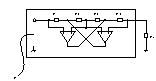
\includegraphics[width=\textwidth]{gyrator_n}
\caption{图~\ref{fig_gyrator}在Windows系统上,用FidoCad打开的绘图。}
\label{fig_gyrator_n}
\end{figure}

对比原FidoCad\index{FidoCad},一个重要的区别就是FidoCadJ可以在输出文件中保存一些配置提示。这是使用\lstinline!FJC!\index{FJC}命令,并通常把它置于文件的最前面。下面段落将描述这些示例。

%======================================= 3级标题
\subsection{层设置}

扩展命令\lstinline!FJC L!\index{FJC L}用于定义层颜色和层透明度,如果用户改变了相应的设置,就会在保存的绘图文件中含有以下命令行:
\begin{lstlisting}
FJC L n xxxx yy
\end{lstlisting}
其中,$n$表示层号(整数,取值范围为[0,15]);$xxxx$表示层颜色(32位整数,RGB值:红色为16-23位,绿色为8-15位,蓝色为0-7位);$yy$表示层透明度(单精度浮点数,0.0表示完全透明~1.0表示完全不透明)。

扩展命令\lstinline!FJC N!\index{FJC N}用于定义层名称,如果用户改变了相应的设置,就会在保存的绘图文件中含有以下命令行:
\begin{lstlisting} 
FJC N n aaaaa
\end{lstlisting}
其中,$n$表示层号(整数,取值范围为[0,15]);{\tt aaaa}表示层名称。

如果用户未改变层设置,绘图文件中不会含有上述扩展命令。此时,FidoCadJ使用默认的层设置。

%======================================= 3级标题
\subsection{电气连接点设置}

扩展命令\lstinline!FJC C!\index{FJC C}用于定义电气连接点的大小,如果用户改变了相应的设置,就会在保存的绘图文件中含有以下命令行:
\begin{lstlisting}
FJC C aaaa
\end{lstlisting}
其中,$aaaa$表示电气连接点直径(正双精度浮点数,单位为FidoCadJ的逻辑单位)。

如果用户未改变电气连接点设置,绘图文件中不会含有上述扩展命令。此时,FidoCadJ使用默认的电气连接点设置。

%======================================= 3级标题
\subsection{线条宽度}

The stroke width for the ``pen'' used during the drawing of electrical schematics can be modified. FidoCadJ adopts the command \lstinline!FJC A!\index{FJC A} to specify the stroke width of the lines, ovals, B�zier, splines, rectangles and polygons. The width can be a double precision constant.
扩展命令\lstinline!FJC A!\index{FJC A}用于定义绘制原理图时使用的线条宽度(双精度浮点数,包括绘制直线、矩形、多边形、椭圆形、贝塞尔曲线和样条曲线)\footnote{在老版本的FidoCadJ中,对于直线(如绘制直线、矩形和多边形)和曲线(如绘制椭圆形和贝塞尔曲线)的线条宽度分别使用扩展命令\lstinline!FJC A!\index{FJC A}和\lstinline!FJC B bbbb!\index{FJC B}指定。但是,从0.23.6版本开始,已经淘汰了这种做法,并把它们统一起来了。},如果用户改变了相应的设置,就会在保存的绘图文件中含有以下命令行:
\begin{lstlisting}
FJC A aaaa
\end{lstlisting}
其中,$aaaa$表示线条宽度(逻辑单位)。

如果用户未改变线条宽度的设置,绘图文件中不会含有上述扩展命令。此时,FidoCadJ使用默认的线条宽度值(0.5个逻辑单位)。

%======================================= 2级标题
\section{语法容错}

FidoCadJ设计有语法容错\index{error tolerance}功能,可以读取非命令行或有语法错误的命令行。然而,应用程序不可能纠正这些错误(除非该应用程序具有魔力\index{crystal ball}),只是简单地跳过这些错误的命令行(保存时会删除这些错误的命令行)。

命令行中缺少层号参数的语法错误是个例外,FidoCadJ并不把它当成错误的命令行,而把它默认为0层\index{layer}(原理图层),这样处理是为了兼容FidoCad\index{FidoCad}。

%======================================= 2级标题
\section{库文件格式}

库文件的格式很简单,请看以下示例:

\begin{lstlisting} 
[FIDOLIB Librairie de base]
{Syboles de base}
[000 Terminal]
LI 100 100 102 100
EV 102 98 106 102
[010 Terminal +]
LI 100 100 102 100
EV 102 98 106 102
LI 103 100 105 100
LI 104 99 104 101
[020 Terminal -]
LI 100 100 102 100
EV 102 98 106 102
LI 103 100 105 100
...
\end{lstlisting} 
第一行定义库的名称(在方括号\index{square brackets}中,以FIDOLIB\index{FIDOLIB}开头,后面为库的名称,中间以空格隔开)。第二行定义宏元件类型名称(在花括号中),表示接下来定义的宏元件的类型。

每个宏元件定义有头\index{header}(在方括号中)和一系列命令组成。头是由特定的\emph{宏元件名称}(在库中的唯一编码)和\emph{宏元件描述}组成。宏元件名称可以用于FidoCadJ脚本,而宏元件描述可以帮助用户概览库中所有的宏元件\index{macro}。命令就是FidoCadJ的绘图命令,命令中的坐标点(100,100)为宏元件的原点,当调用宏元件绘图时,这个点将作为参考点。在FidoCadJ脚本中,宏元件用{}”library.macro”定义,并用MC\index{MC}命令调用。

一个宏元件的定义中总是可以调用另一个宏元件,但不要进行递归\index{recursion}调用(即在宏元件的定义中调用它自己)。

在库文件中,\textit{不能包括}任何关于FidoCadJ的配置信息。换句话说,库文件中\textit{不能}出现FJC\lstinline!FJC!\index{FJC}命令。

%======================================= 2级标题
\section{标准库}

FidoCadJ包含FidoCad\index{FidoCad}传统支持的2个库(即“Stand library”\index{standard library}和“PCB Footprints”\index{PCB library}库),即为FidoCadJ的标准库,默认加载它们。

然而通过“文件/选项/启动”设置加载库文件夹,可以覆盖或增加FidoCadJ的默认加载库。如果设置的加载库文件夹中存在一个名称为\lstinline!FCDstdlib.fcl!的文件,它将替换标准库;如果存在一个名称为\lstinline!PCB.fcl!的文件,它将替换PCB库;如果存在扩展名为\lstinline!fcl!的其它文件,将作为其它库一起被载入。

%======================================= 1级标题
\chapter{总结}

在前面章节中,我们已经介绍过了如何使用FidoCadJ来绘制一张电路原理图和一张简单的PCB图。目前阶段,读者应该可以使用FidoCadJ进行绘图了。

然而,FidoCadJ不仅可以用于电子电路的绘图,也可以用于任何其它类型的2D绘图,并且多数2D类型的绘图可以找到其相关的特定库。

FidoCadJ是自由程序,其优点是:完全开放给它的用户社区。如此,您的反馈对我很重要(至少让我了解到该项目是否值得继续开发以及它的发展方向)。请和我联系吧!随时欢迎您加入到SourceForge论坛并致力于FidoCadJ项目\footnote{\href{https://sourceforge.net/projects/fidocadj/forums/forum/997486}{https://sourceforge.net/projects/fidocadj/forums/forum/997486}}。

\appendix

%======================================= 1级标题
\chapter{操作系统上的特殊性} \label{specifics} 

%======================================= 2级标题
\section{MacOSX系统}

Macintosh的用户(比如我)对早期版本的FidoCadJ提出的最多的批评是应用程序在MacOSX系统上集成的不好。从0.21.1版本开始,FidoCadJ为此做了努力,以更好地符合MacOSX系统应用程序的外观和理念。这就导致了FidoCadJ运行于MacOSX系统上时出现了一些细微的差异:
\begin{itemize}
\item 当运行完整的应用程序(运行FidoCadJ.app\index{FidoCadJ.app}而不是FidoCadJ.jar\index{fidocadj.jar})时,FidoCadJ默认使用Quaqua\footnote{\href{http://www.randelshofer.ch/quaqua/}{http://www.randelshofer.ch/quaqua/}}\index{Quaqua} LookAndFeel。当在老式的机器上运行应用程序时,Quaqua可能会降低其运行性能,此时,通过Preferences菜单设置,可以禁用它。
\item 菜单工具栏显示在MacOSX系统应用程序窗口的合理位置上(应用程序窗口的顶部)。
\item 菜单项{}“Preferences”和{}“关于FidoCadJ”出现在MacOSX系统应用程序窗口的合理位置上(FidoCadJ菜单的下面)。
\item 应用程序会告知MacOSX系统,它可以打开扩展名为\lstinline!.fcd!的文件,并让这类文件关联一个特定的图标,让人一眼就能看出这是用FidoCadJ打开的文件。
\end{itemize}

%======================================= 3级标题
\subsection{下载并运行FidoCadJ}
FidoCadJ可以运行在10.3.9(豹\index{Panther})版本及最新版本的MacOSX\index{MacOSX}系统上。这是因为,运行FidoCadJ最低需要Java 1.5版本,苹果曾经在10.3.9版本的操作系统中提供Java 1.5。由于市场原因,苹果似乎并不想在最新版本的MacOSX\index{MacOSX}系统中提供Java。然而,Java是运行FidoCadJ必不可少的基础部件,因此,您需要下载并安装它。顺便说下,苹果不允许在它的应用商店\index{App Store}中发布基于Java或GPL授权的软件,这就是FidoCadJ不可能移植到iPad\index{iPad}和iPhone\index{iPhone}上的一个最重要的原因。

虽然在其它操作系统上,您可以直接使用Java打包文件\lstinline!fidocad.jar!,然而在MacOSX系统上,您需要使用专门定制的FidoCadJ应用程序(磁盘镜像)。该应用程序所有的一切看起来就是一个本系统的应用程序。您可以从以下链接下载到运行在MacOSX系统上的FidoCadJ应用程序的磁盘镜像,\\
 {\small \href{http://sourceforge.net/projects/fidocadj/files/FidoCadJ_MacOSX.dmg/download}{http://sourceforge.net/projects/fidocadj/files/FidoCadJ\_ MacOSX.dmg/download}}\\
然后您可以打开它,把\lstinline!FidoCadJ.app!移动到\lstinline!Applications!文件夹中,在这里,您可以像其它MacOSX系统上的应用程序一样地使用它。想要卸载FidoCadJ,只要把\lstinline!FidoCadJ.app!拖进垃圾桶。

%======================================= 2级标题
\section{Linux系统}

\label{installazione_linux} \textsl{Roby IZ1CYN编写}\\

首先:必须安装SUN\index{Sun} JRE\index{JRE}6和/或OpenJDK\index{OpenJDK} 6 JRE\index{JRE}(或是应用程序说明的可使用的早期版本)。\ref{inst_testo}~章节将介绍终端命令行方式安装程序的方法。\ref{inst_grafica}~章节将介绍图形环境中安装程序的方法。Java运行时环境配置的好坏,决定了FidoCadJ的运行性能。\footnote{\textit{请}相信我,如果你喜欢的Linux发行版运行Java很不稳定,应该就是这个原因!}

%======================================= 3级标题
\subsection{通用的终端安装方法}

\label{inst_testo} 使用\lstinline!wget!命令下载程序:

%\lstset{language=plain,%
%	basicstyle=\tiny\ttfamily}

\begin{lstlisting}
$ wget http://downloads.sourceforge.net/project/fidocadj/fidocadj.jar?use_mirror=garr
--00:48:18--  http://downloads.sourceforge.net/project/fidocadj/fidocadj.jar?use_mirror=garr
           => `fidocadj.jar?use_mirror=garr'
Resolution of downloads.sourceforge.net is being done... 216.34.181.59
Connection to downloads.sourceforge.net|216.34.181.59:80... connected.
HTTP request sent, waiting for answer... 302 Found
URL: http://garr.dl.sourceforge.net/project/fidocadj/fidocadj.jar
--00:48:24--  http://garr.dl.sourceforge.net/project/fidocadj/fidocadj.jar
           => `fidocadj.jar'
Resolution of garr.dl.sourceforge.net is being done... 193.206.140.34
Connection to garr.dl.sourceforge.net|193.206.140.34:80... connected.
HTTP request sent, waiting for answer... 200 OK
Length: 343,207 (335K) [application/java-archive]

100%[====================================>] 343,207      422.48K/s             

00:48:30 (420.55 KB/s) - "fidocadj.jar" saved [343207/343207]
$
\end{lstlisting}
\lstset{
	basicstyle=\small\ttfamily}

另外,如果上面的方法行不通,您也可以使用任何浏览器从下面的URL下载文件:\\
\href{http://sourceforge.net/projects/fidocadj/files/fidocadj.jar/download}{http://sourceforge.net/projects/fidocadj/files/fidocadj.jar/download}
并把文件保存到\lstinline!/home/!目录中。

创建一个新目录(首先我们要使用\lstinline!su!或\lstinline!sudo -s!命令成为超级用户\index{superuser},然后才能创建新目录):

\begin{lstlisting}
# mkdir /usr/bin/fidocadj
\end{lstlisting}

把下载的文件移到该目录中(把\lstinline!<user>!替换成登录账户的用户名,那里有已下载的文件):

\begin{lstlisting}
# mv /home/<user>/fidocadj.jar /usr/bin/fidocadj
\end{lstlisting}

把文件设置成可执行的。

\begin{lstlisting}
# chmod +x /usr/bin/fidocadj/fidocadj.jar
\end{lstlisting}

一定不要忘记切换回普通用户:

\begin{lstlisting}
# exit
\end{lstlisting}

现在,我们可以执行程序了:

\begin{lstlisting}
$ /usr/bin/fidocadj/fidocadj.jar
\end{lstlisting}

%======================================= 3级标题
\subsection{图形安装方法}
\label{inst_grafica}
以Ubuntu\index{Ubuntu} 8.04为例,展示图形化安装方法,在新版本的Ubuntu系统上安装的差别不会很大。

\begin{itemize}
\item{用浏览器下载文件,也可以使用Gwget或类似工具下载文件。}

\item{通过文件管理器创建以下目录(如果菜单中没有文件管理器(Nautilus或Konqueror或\dots),需要用root权限加载一个,例如用\lstinline!sudo nautilus!命令从控制台启动Nautilus):
\begin{lstlisting}
/usr/bin/fidocadj
\end{lstlisting}
把刚下载的文件移到该目录中。下载的文件可能在:
\begin{lstlisting}
/home/<user>/
\end{lstlisting}}

\begin{figure}
\centering
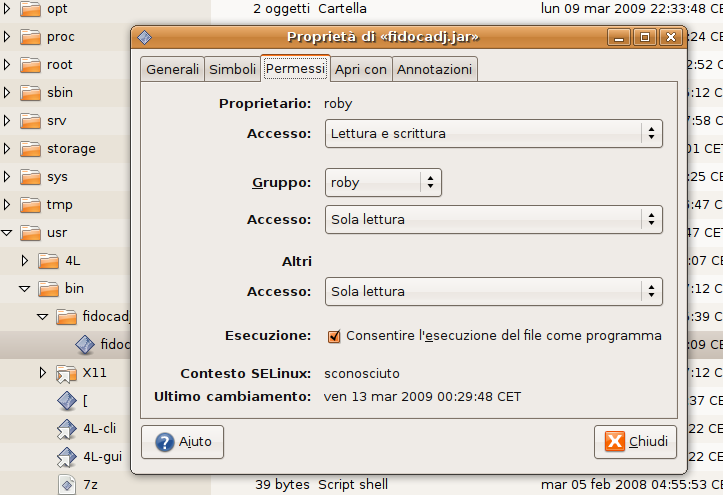
\includegraphics[width=.8\textwidth]{permessi}
\caption{Ubuntu\index{Ubuntu} 8.04系统,文件权限设置。}
\label{fig_permessi}
\end{figure}

\item{在文件上右击,会弹出菜单,其中我们打开“rights”分页,在“Allow the execution of the file as a program”前面选项框中打勾,见图~\ref{fig_permessi}~所示。}

\begin{figure}
\centering
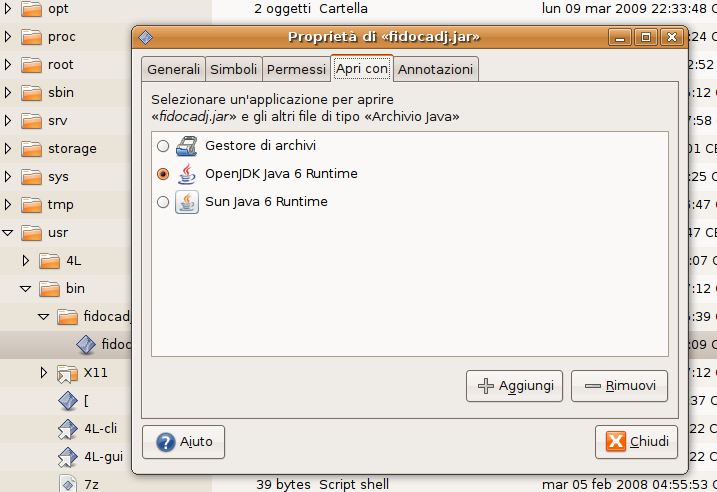
\includegraphics[width=.8\textwidth]{java6}
\caption{Ubuntu\index{Ubuntu} 8.04系统,设置执行程序使用的Java虚拟机。}
\label{fig_java6}
\end{figure}

\item {我们可以打开“Open as”分页,并选择“OpenJDK Java6 Runtime”或“Sun Java6Runtime”,见图~\ref{fig_java6}~所示。}

\item {点击“Close”按钮,现在,我们准备运行FidoCadJ:双击可执行文件即可运行,或者我们可以把它加入到主菜单。加入主菜单,只需要运行命令\lstinline!/usr/bin/fidocadj/fidocadj.jar!。}
\end{itemize}

%======================================= 2级标题
\section{Windows系统}
从0.23版本开始,FidoCadJ可以识别出Windows系统,并且会使用该系统的LookAndFeel。

%======================================= 3级标题
\subsection{下载并运行FidoCadJ}
通常,如果您的Windows系统中已经安装了Java,您只需要下载\lstinline!fidocadj.jar!文件,双击它即可运行。如果您的Windows系统把下载的jar文件识别成一个类似\lstinline!zip!的打包文件,那么可能系统中未安装Java。Oracle允许您自由下载和安装最新版本的Java运行时:\\ \href{http://www.java.com/it/download/}{http://www.java.com/it/download/}

%\manualmark 
%\markboth{\spacedlowsmallcaps{\indexname}}% 
%{\spacedlowsmallcaps{\indexname}} 
%\refstepcounter{dummy} 
%\pagestyle{scrheadings} 
%\addcontentsline{toc}{chapter}{\tocEntry{\indexname}} 
\printindex 
\cleardoublepage
\thispagestyle{empty}
\mbox{ }
\vfill
该手册是在MacOSX系统上使用\textsc{pdf}\LaTeX\ 编写的。列表由\href{http://www.ctan.org/tex-archive/macros/latex/contrib/listings/}{listings}包编译生成。\href{http://www.ctan.org/tex-archive/graphics/pgf/}{pgf}包用于生成图~\ref{fig_schema}~。所有其它用到的包来自CTAN档案。

%This work has been composed with the \emph{Palatino} font, by Hermann Zapf. 


\end{document}